%% Template for Physical Review D papers
%% Adapted from thesis Chapter F: cDVGAN for realistic glitch synthesis

\documentclass[reprint,nofootinbib,amsmath,amssymb,aps,floatfix]{revtex4-2}

% Math packages
\usepackage{bm}
\usepackage{dcolumn}

% Graphics and figures
\usepackage{graphicx}
\usepackage{subcaption}
\usepackage{placeins}

% Tables
\usepackage{booktabs}
\usepackage{multirow}

% Formatting
\usepackage{xspace}
\usepackage{xcolor}
\usepackage[colorlinks=true,linkcolor=blue,citecolor=blue,urlcolor=blue]{hyperref}
\usepackage[font=small,labelfont=bf,textfont=it]{caption}
\usepackage{pifont}
\newcommand{\cmark}{\ding{51}}
\newcommand{\xmark}{\ding{55}}

\begin{document}

\preprint{APS/123-QED}

\title{Realistic Synthesis of Gravitational-Wave Detector Glitches using Class-Conditional Derivative Generative Adversarial Networks}

\author{Tom Dooney$^{1,2}$}
\author{Mees de Boer$^{2}$}
\author{Harsh Narola$^{1,2}$}
\author{Melissa Lopez$^{1,2}$}
\author{Stefano Bromuri$^{3}$}
\author{Daniel Stanley Tan$^{3}$}
\author{Chris Van Den Broeck$^{1,2}$}

\affiliation{$^1$Nikhef, Science Park 105, 1098 XG Amsterdam, The Netherlands}
\affiliation{$^2$Institute for Gravitational and Subatomic Physics (GRASP), Utrecht University, Princetonplein 1, 3584 CC Utrecht, The Netherlands}
\affiliation{$^3$Faculty of Science, Open Universiteit, Valkenburgerweg 177, 6419 AT Heerlen, The Netherlands}

\date{\today}

%% Abstract
\begin{abstract}
Gravitational-wave detectors such as LIGO, Virgo, and KAGRA are highly sensitive instruments susceptible to numerous noise sources. 
Short-duration transient noise events, known as glitches, pose a particular challenge for data analysis pipelines as they can mimic or obscure astrophysical signals. 
We present GlitchGAN, a class-conditional generative model, built upon the Conditional Derivative GAN (cDVGAN) architecture, that is capable of synthesizing realistic glitches directly in the time domain. 
The model is trained on high-quality reconstructions of seven common glitch types observed during LIGO's third observing run (O3): Blip, Fast Scattering, Koi Fish, Low-Frequency Burst, Scattered Light, Tomte, and Whistle.
% We demonstrate that cDVGAN generalizes effectively across this diverse glitch population, learning continuous class-conditional morphologies that interpolate between glitch types.
We show that GlitchGAN generalizes effectively, learning to reproduce a diverse and physically consistent glitch space directly from these reconstructions. 
Moreover, because the model is conditioned on glitch class, it can generate \textit{hybrid} or transitional glitch morphologies by interpolating across the class-conditioning vector after training.
% Synthetic glitches are validated against real data using unsupervised UMAP embeddings and the Gravity Spy classifier, showing substantial overlap in latent space and correct classification rates exceeding 90\% for well-characterized classes.
Synthetic glitches are validated against real glitches using unsupervised UMAP embeddings and the Gravity Spy classifier, widely used in the GW community for glitch classification.
The UMAP analysis shows substantial overlap between real and synthetic samples in the reduced latent space, while Gravity Spy classifies the majority of GlitchGAN's synthetic glitches as the correct class. 
We further highlight a critical limitation of magnitude-only spectrograms: classifiers operating on $Q$-transforms can confidently misclassify physically unrealistic glitches from less robust models, underscoring the need for complementary validation methods that preserve phase information.
% Our results demonstrate the viability of deep generative models for producing realistic synthetic glitches suitable for detector simulations, mock data challenges, and pipeline validation.
% At the same time, these results reveal the limitations of relying solely on $Q$-transform–based (magnitude spectrogram) representations, as employed by classifiers such as Gravity Spy, which can confidently misclassify unrealistic samples from less robust generative models. 
% They highlight the critical role of phase information for accurately capturing glitch morphology, which is discarded in standard $Q$-transforms used for glitch classification, and underscore the need for complementary unsupervised validation methods to achieve more reliable glitch characterization.
\end{abstract}

\maketitle

%% ============================================================================
%% MAIN DOCUMENT
%% ============================================================================

\section{Introduction}

The direct detection of gravitational waves (GWs) by the LIGO \cite{LIGO_paper} and Virgo \cite{VIRGOpaper} interferometers has opened a new observational window on the universe, enabling measurements of compact binary coalescences and other cataclysmic astrophysical events~\cite{GWTC_3_catalog}.
The extreme sensitivity required for these detections, however, renders the instruments equally susceptible to instrumental and environmental noise sources~\cite{LIGO_O3_detector_characterization}.
Among these, short-duration transient noise artefacts known as \textit{glitches}~\cite{LIGO_second_third_detchar, Virgo_detchar_O3, Kagra_detchara} represent a persistent challenge for data analysis pipelines.
Glitches exhibit remarkable morphological diversity---ranging from impulsive millisecond-duration events to extended, dispersive features spanning several seconds---and can mimic or obscure astrophysical signals~\cite{abbott2018effects, blackburn2008lsc, abbott2016characterization}.
When a glitch overlaps with a genuine GW signal it can significantly bias parameter estimation~\cite{pankow2018mitigation, PE_glitch_1, PE_glitch_2}, and approximately 25 of the $\sim\!90$ confident detections to date required some form of glitch mitigation~\cite{GWTC_3_catalog, pankow2018mitigation, BNS_1, BNS_2, BNS_BBH_1, BNS_BBH_2}.
With the anticipated sensitivity improvements of next-generation detectors such as Einstein Telescope \cite{ET_paper} and Cosmic Explorer \cite{Cosmic_expl}, the rate and impact of glitches are expected to increase substantially~\cite{Detchar_nextgen_glitch}.

The ability to synthesize accurate and realistic glitch populations is therefore of growing importance.
Such capability enhances the realism of detector simulations and supports software injection campaigns~\cite{Abadie_2010_injection_1, Abadie_2010_injection_2, Biwer_2017_inject, Virgo_detchar_O3}, enabling more rigorous testing and validation of GW detection pipelines and parameter estimation algorithms.
Realistic synthetic glitches are also essential for the construction of mock data challenges (MDCs) and for data augmentation in machine learning-based glitch classification systems.

Generative adversarial networks (GANs)~\cite{Goodfellow:2014upx}, wherein a generator and discriminator are trained in an adversarial minimax game, have established themselves as a powerful framework for learning complex high-dimensional data distributions.
Wasserstein GANs (WGANs)~\cite{wGAN_paper} improve training stability by replacing the Jensen--Shannon divergence with the Wasserstein-1 distance, and the gradient penalty variant (WGAN-GP)~\cite{wGAN_GP_paper} further stabilizes optimization by enforcing a Lipschitz constraint on the discriminator.
Conditional extensions~\cite{Mirza_2014} allow the generator to be steered towards a target class, enabling multi-class synthesis within a single model.

Generative models have been applied broadly within GW data analysis.
Conditional autoencoders have been used to generate accurate waveform models for non-spinning binary black hole mergers at a fraction of the computational cost of traditional methods~\cite{Liao:2021vec}, while GANs have been shown to reproduce distributions of core-collapse supernova GW signals~\cite{PhysRevD.110.104055}.
For glitch synthesis, GANs have been used to augment spectrogram-based datasets for downstream classification tasks~\cite{GAN_spec_best, Jade_Powell_paper}.
The \textit{gengli} glitch generator~\cite{GENGLI, GENGLI_2} demonstrated that a WGAN trained on Blip glitches extracted from detector backgrounds using BayesWave~\cite{BayesWave} can successfully learn their underlying time-domain distribution, providing a useful framework for simulations and MDCs.
McGANn~\cite{McGinn_2021} extended this to a conditional GAN capable of simultaneously synthesizing five waveform classes analogous to GW bursts, with class interpolation enabling hybrid morphologies.
Powell et al.~\cite{Jade_Powell_paper} further extended this to a broader glitch class space by training separate GANs on $Q$-scan representations of each Gravity Spy class.
However, extending this holistic approach to a single model operating directly in the time domain remains unexplored, despite its advantages in preserving phase information and enabling direct use of time-series data in MDCs and detection pipelines.

In previous work~\cite{dooney2022dvgan, cdvgan}, we introduced DVGAN and its conditional extension cDVGAN, a modified GAN architecture featuring an auxiliary discriminator that operates on the time derivative of training signals.
This derivative discriminator was shown to improve both training stability and sample fidelity compared to standard WGAN-GP counterparts.
While cDVGAN demonstrated the ability to conditionally generate multiple waveform classes within a single model---including proxy Blip and Tomte glitch classes alongside simulated BBH signals---these models were validated only on simplified, preprocessed datasets not representative of the realistic glitch space observed in GW detectors.
Whether this approach generalizes to reconstructions of real LIGO glitches, which are inherently more complex and impose no assumptions about waveform smoothness, remained an open question.

The principal obstacle to realistic time-domain glitch synthesis has been the availability of high-quality training data.
BayesWave~\cite{BayesWave}, the state-of-the-art method for reconstructing glitches from detector data, imposes a smoothness prior through its Gabor-Morlet wavelet basis, is computationally expensive, and converges unreliably across all glitch morphologies.
These limitations make it impractical to construct the large-scale, diverse training datasets required for deep generative models; consequently, earlier time-domain models trained on BayesWave reconstructions may not capture the full complexity of real glitch morphologies.

The emergence of DeepExtractor~\cite{DeepExtractor_paper}---a deep learning U-Net framework for time-domain glitch reconstruction---has changed this landscape.
DeepExtractor provides fast, high-fidelity reconstructions that preserve both amplitude and phase information without imposing waveform smoothness assumptions, achieving a $10{,}000\times$ speed-up over BayesWave in realistic simulations.
This enables the construction of large-scale, diverse training datasets representative of real detector noise across many glitch classes.

In this paper, we evaluate GlitchGAN's capability to generate time-domain glitches from a class space that is substantially larger, more realistic, and more complex than the well-behaved proxy datasets examined in prior work.
The training dataset is constructed from DeepExtractor reconstructions of seven of the most common glitch classes observed during LIGO's O3: Blip, Fast Scattering, Koi Fish, Low-Frequency Burst, Scattered Light, Tomte, and Whistle.
We first validate the quality of the reconstructed training data using the Gravity Spy classifier~\cite{Zevin_2017, GspyO4} and unsupervised UMAP embeddings~\cite{McInnes_2018}, establishing a baseline against which synthetic glitches can be assessed.
We then train GlitchGAN on this dataset and evaluate whether a single conditional model can reproduce the full morphological diversity of this realistic glitch population.

The results demonstrate that GlitchGAN captures much of the morphological diversity across all seven classes, with substantial overlap between real and generated distributions in the UMAP latent space and with the majority of synthetic glitches correctly identified by Gravity Spy.
We further highlight a fundamental limitation of magnitude-only time-frequency representations as validation tools.
When classifying physically unrealistic glitches produced by a diffusion-based comparison model~\cite{diffusionOriginal}, Gravity Spy assigns them to the correct class with high confidence despite their clear inconsistency with real data in the time domain---because the $Q$-transform used by Gravity Spy discards phase information entirely.
This underscores the necessity of complementary, phase-preserving validation methods such as UMAP applied directly to time-domain waveforms.

The remainder of the paper is organized as follows:
Section~\ref{sec:data} describes the curation and preparation of our training dataset.
Section~\ref{sec:methods} details the GlitchGAN architecture (based on cDVGAN) and training procedure.
Section~\ref{sec:results} presents validation results across multiple metrics.
Finally, Section~\ref{sec:discussion} discusses the implications of our findings and opportunities for future work.

\begin{figure*}[t]
\centering
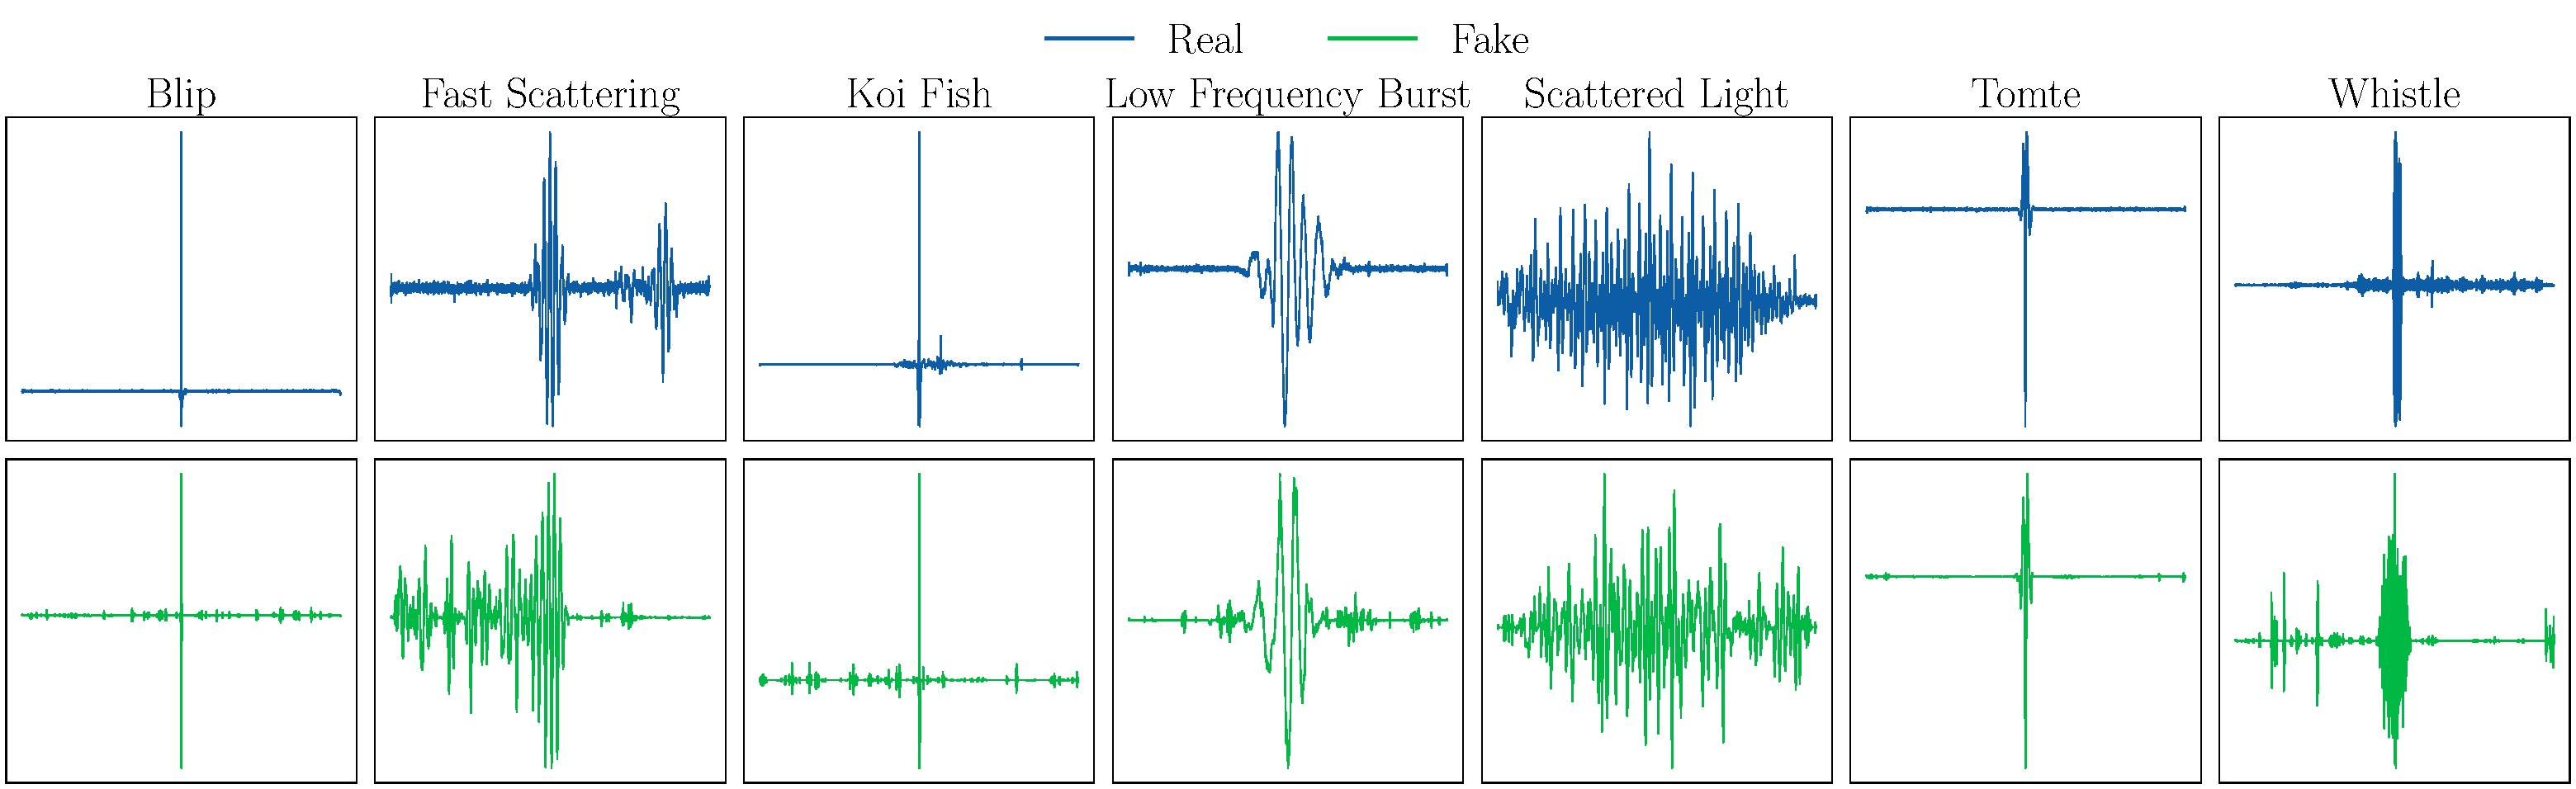
\includegraphics[width=0.8\linewidth]{figures/real_vs_generated_glitch_waveforms_2.pdf}
\caption[Real and generated glitch waveforms for seven classes]{
Comparison between real and synthetic glitch waveforms across the seven glitch classes used for training.
\textbf{Top:} Real glitches reconstructed with DeepExtractor.
\textbf{Bottom:} Synthetic glitches generated by GlitchGAN after training.
Each panel shows one representative glitch per class, illustrating the model's ability to reproduce distinct morphological features observed in the real data.}
\label{fig:real_vs_generated_waveforms}
\end{figure*}

% \section{Background: Glitches and Previous Synthesis Approaches}
% \label{sec:background}

% \subsection{Nature and characterization of detector glitches}

% Glitches are transient noise events typically lasting from tens of milliseconds to a few seconds.
% They exhibit remarkable morphological diversity, ranging from impulsive sharp features to extended, dispersive phenomena.
% The Gravity Spy citizen science project \citep{Zevin_2017} has enabled classification of millions of glitches, identifying over 20 distinct morphological classes.
% The most common classes include Blip, Tomte, Whistle, Low-Frequency Burst, Scattered Light, Koi Fish, and Fast Scattering---the seven classes we focus on in this work.

% Different glitch morphologies often reflect distinct physical origins:
% Blips are typically impulsive events, possibly related to sudden mechanical motion or electronic transients.
% Whistles are characterized by narrow-band, time-dispersive features suggesting coupling from seismic or thermal noise into the laser frequency.
% Low-Frequency Bursts represent broadband energy at frequencies below 100~Hz and may arise from various mechanical or thermal transients.
% Scattered Light features result from acoustic reverberation of scattered photons, while Fast Scattering represents higher-order scattering interactions.
% Koi Fish exhibit distinctive ``V''-shaped or ``U''-shaped lofting patterns in spectrograms, possibly indicating nonlinear coupling phenomena.
% Tomte glitches show complex, extended structures with multiple frequency components.

% Understanding and characterizing this diversity is critical because not all glitches are created equal in their impact on astrophysical searches.
% An accurate glitch population model is essential for:
% \begin{enumerate}
% \item Validating detector characterization algorithms
% \item Assessing the impact of glitches on parameter estimation
% \item Testing robustness of detection pipelines to instrumental noise
% \item Developing effective glitch mitigation and subtraction strategies
% \end{enumerate}

% \subsection{Prior approaches to glitch synthesis}

% Generative models have recently emerged as promising tools for synthesizing realistic glitch populations.
% Early approaches \citep{Powell_2019, Powell_2022} trained separate Bidirectional GANs (BiGANs) or other GAN architectures for each glitch class in the $Q$-scan spectrograms domain.
% While this approach demonstrated viability, it operates in the spectrogram (magnitude) domain, discarding phase information that is crucial for accurate waveform representation.

% Subsequent work explored diffusion-based generative models and VAE-GAN combinations, with varying degrees of success.
% A key limitation of prior work has been reliance on either (i) preprocessed glitches with substantial temporal smoothing, (ii) BayesWave reconstructions that impose strong phenomenological assumptions about waveform structure, or (iii) spectrogram-domain representations that lose phase information.

% The development of DeepExtractor \citep{DeepExtractor_paper} changed this landscape by providing an unsupervised deep learning approach for extracting glitch time-domain waveforms directly from detector data, without assumptions about the form of the underlying signal.
% DeepExtractor reconstructions preserve both amplitude and phase information, enabling much higher-fidelity training data for generative models.

% Our work is the first to demonstrate that a single class-conditional model can effectively learn to generate multiple complex glitch classes in the time domain from DeepExtractor reconstructions, leveraging the full morphological diversity available in the training data.

\FloatBarrier
\section{Data}
\label{sec:data}


\subsection{Data curation}

We construct our training dataset using DeepExtractor reconstructions of real LIGO glitches from Grave Spy.
To ensure high-quality, morphologically representative samples, we apply strict selection criteria:

\begin{enumerate}
\item
Gravity Spy classification confidence $\sigma_{\text{GS}} \geq 0.9$ (strong morphological match to training class)

\item
Signal-to-noise ratio (SNR) $\geq 15$ (sufficient amplitude to minimize reconstruction artifacts)

\item
Detectors: LIGO Hanford (H1) and Livingston (L1)

\item
Observing runs: O3a and O3b

% \item Resampled to 8192 samples (corresponding to 2 seconds at 4096~Hz sampling rate)
\item Reconstruct with DeepExtractor a 2-second window centered on the glitch trigger time at a sampling rate of 4096~Hz, yielding 8192 samples per waveform

\end{enumerate}

Glitch classes included: Blip, Fast Scattering, Koi Fish, Low-Frequency Burst, Scattered Light, Tomte, and Whistle.
These seven classes collectively span wide time and frequency ranges, encompassing much of the morphological variability relevant to transient instrumental noise.
While it is a common glitch class, we exclude the Extremely Loud class because its characterization is dominated by exceptionally high SNR rather than distinctive morphology, making it a poor target for generative modeling.

% The Extremely Loud threshold and other class boundaries defined by Gravity Spy naturally partition the morphological space.

\subsection{Dataset Preprocessing}

Our goal was to obtain approximately 5,000 samples per class (1,250 per detector per observing run) under the selection criteria above.
Unfortunately, data availability constraints limited acquisition for some classes.
Fast Scattering yielded only 2,774 samples, and Low-Frequency Burst provided 4,316 samples.
The total curated dataset contained 31,511 samples.

To mitigate training instabilities from class imbalance, we applied bootstrap resampling (sampling with replacement) to oversample all classes to 5,000 samples each, yielding a balanced training set of 35,000 total samples.
Dataset composition by detector, observing run, and class is detailed in Table~\ref{tab:glitch_pivot_summary}.
Before training, all reconstructed time series are normalized to the range $[-1, 1]$, followed by subtracting the mean.
% \begin{enumerate}
% \item Normalized to the range $[-1, 1]$
% \item Mean-subtracted 
% % \item Resampled to 8192 samples (corresponding to 2 seconds at 4096~Hz sampling rate)
% \end{enumerate}
This normalization constrains the generative model to operate at a single effective SNR scale, but generated samples can be rescaled post-generation to any desired SNR for downstream applications.

\begin{table}[ht]
    \centering
    \caption{Composition of the curated glitch dataset. Number of samples per class, detector (H1: Hanford, L1: Livingston), and observing run (O3a, O3b). Classes are bootstrapped to 5000 samples each for balanced training.}
    \label{tab:glitch_pivot_summary}
    \begin{tabular}{l rrrr}
    \toprule
    \multirow{2}{*}{Glitch Class} & \multicolumn{2}{c}{H1} & \multicolumn{2}{c}{L1} \\
    \cmidrule(lr){2-3} \cmidrule(lr){4-5}
    & O3a   & O3b   & O3a   & O3b   \\
    \midrule
    Blip                  & 1246 & 1247 & 1245 & 1243 \\
    Fast\_Scattering      & 143  & 143  & 1244 & 1244 \\
    Koi\_Fish             & 1247 & 1248 & 1243 & 1247 \\
    Low\_Frequency\_Burst & 1246 & 1246 & 912  & 912  \\
    Scattered\_Light      & 1236 & 1243 & 1246 & 1248 \\
    Tomte                 & 1031 & 1031 & 1247 & 1246 \\
    Whistle               & 1232 & 1232 & 1231 & 1232 \\
    \bottomrule
    \end{tabular}
\end{table}

\section{Methods}
\label{sec:methods}

\subsection{Model architecture: cDVGAN}

cDVGAN~\cite{cdvgan} is a conditional Wasserstein GAN with gradient penalty (WGAN-GP)~\cite{wGAN_paper, wGAN_GP_paper} that augments the standard two-player adversarial game with an auxiliary discriminator applied to the first-order time derivative of signals.
Here we summarise the key components; full layer-by-layer architecture details are given in~\cite{cdvgan}.

\subsubsection{Training objective}

Under the WGAN-GP framework, the discriminator loss is
\begin{equation}
    L_D = \mathbb{E}_{\hat{x}}[D(\hat{x},c)] - \mathbb{E}_{x}[D(x,c)] + \lambda\,\mathbb{E}_{\tilde{x}}\!\left[\left(\|\nabla_{\tilde{x}} D(\tilde{x},c)\|_2 - 1\right)^2\right],
\end{equation}
where $x$ and $\hat{x}$ are real and generated samples respectively, $\tilde{x}$ is a random interpolation between them, and $\lambda = 10$ is the gradient-penalty weight.
The generator is updated to minimise
\begin{equation}
    L_G = -\mathbb{E}_{\hat{x}}[D(\hat{x},c)].
\end{equation}

In cDVGAN a second discriminator $D_\partial$ operates on the first-order derivative $\dot{x} = dx/dt$.
The combined generator loss is
\begin{equation}\label{eq:combined_loss}
    L_G^{\text{cDVGAN}} = -\frac{1}{2}\left(\mathbb{E}_{\hat{x}}[D(\hat{x},c)] + \mathbb{E}_{\dot{\hat{x}}}[D_\partial(\dot{\hat{x}},c)]\right),
\end{equation}
where both discriminators contribute equally.
Each discriminator is updated five times per generator update.

\subsubsection{Generator}

The generator $G$ maps a noise vector $z \sim \mathcal{N}(0, I_{100})$ and a one-hot class vector $c \in \mathbb{R}^7$ to a time series of length 8192.
The class vector is first projected to a 32-dimensional embedding and concatenated with $z$, then passed through a dense layer and reshaped before five successive upsample-and-convolve blocks with batch normalisation and ReLU activations expand the sequence to the target length.

\subsubsection{Discriminators}

Both $D$ and $D_\partial$ are 1D convolutional networks that map an input sequence and a class vector to a scalar critic value.
Class conditioning uses projection~\cite{Mirza_2014}: a learned class embedding is dot-producted with the discriminator's feature vector and added to the scalar output.
$D$ operates directly on the 8192-sample waveform; $D_\partial$ operates on the 8191-sample first-order difference sequence $\dot{x} = x_{t+1} - x_t$.
The derivative discriminator provides additional regularisation by penalising unphysical high-frequency artefacts in generated waveforms~\cite{dooney2022dvgan}.

\subsection{Training procedure}

The model was trained for 500 epochs with a batch size of 64 using the RMSprop optimiser with learning rate $10^{-4}$ for all components.
Training was performed on an NVIDIA A100 GPU (approximately 12 hours).
No hyperparameter tuning was performed for this dataset; the architecture and hyperparameters are identical to those validated in~\cite{cdvgan}, allowing us to assess out-of-the-box generalisation to this more complex and realistic glitch population.

\subsection{Comparison with a diffusion-based model}

As a comparison, we trained a latent Diffusion Transformer (DiT) model adapted for 1D time series.
Full-resolution diffusion proved computationally prohibitive, so we first trained a convolutional autoencoder to compress inputs from $(8192,1)$ to a latent space of $(256,16)$, reducing computational cost by approximately three orders of magnitude while preserving essential morphological structure.
The DiT was then trained in this latent space, with generated samples decoded back to the time domain for evaluation.
This model serves primarily to illustrate the limitation of magnitude-only validation metrics, as discussed in Section~\ref{sec:results}.

\section{Results}
\label{sec:results}

\begin{figure*}[t]
\centering
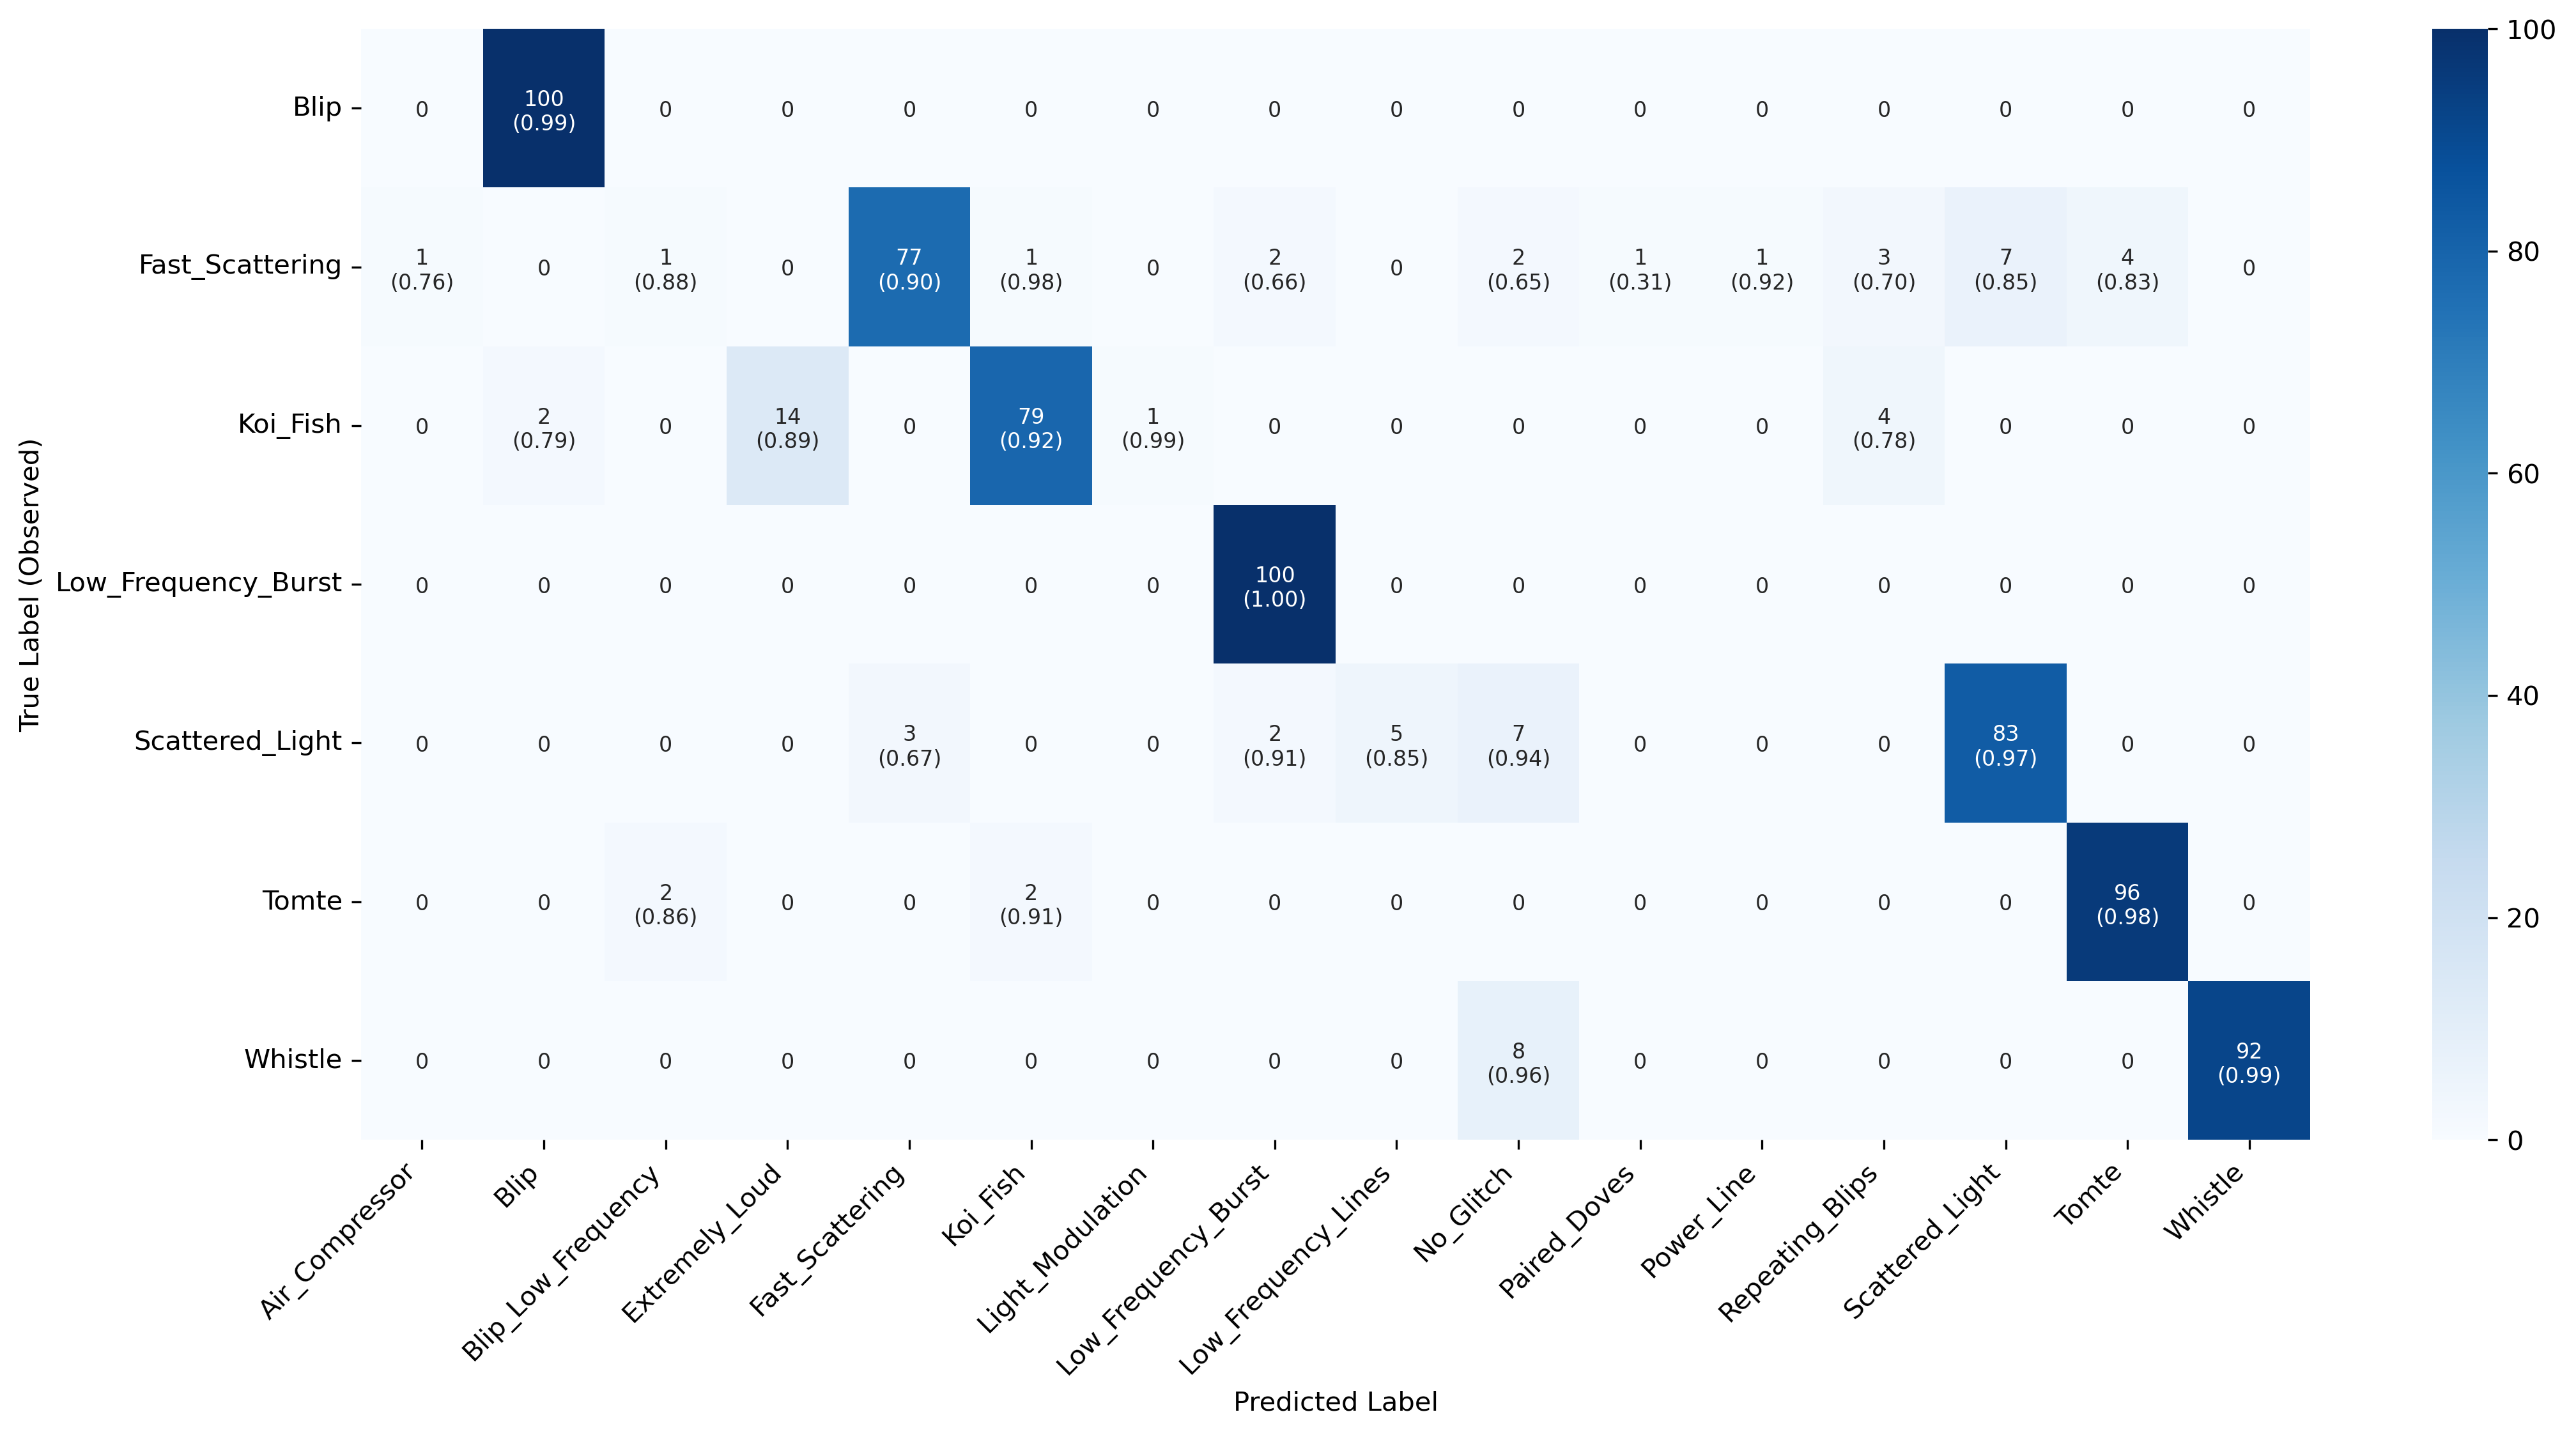
\includegraphics[width=0.8\linewidth]{figures/deepextractor_confusion_matrix.png}
\caption{Confusion matrix for Gravity Spy classification of 100 DeepExtractor reconstructions per class (700 total). Each cell shows the number of predictions with the mean Gravity Spy confidence in brackets.}
\label{fig:de_confusion}
\end{figure*}


\subsection{Validation of DeepExtractor training data}
\label{sec:deepextractor_validation}

Before evaluating GlitchGAN-generated glitches, we first validate the quality of the DeepExtractor reconstructions that form our training dataset.
This serves two purposes: (i) confirming that the reconstructions preserve the morphological characteristics recognized by Gravity Spy, which is a prerequisite for using them as realistic training data; and (ii) establishing a qualitative and quantitative baseline against which to compare the synthetic glitches produced by GlitchGAN.

We reconstruct with DeepExtractor 100 randomly selected glitches from the Gravity Spy dataset according to the criteria in Section \ref{sec:data}, drawing 25 samples per detector (H1, L1) per observing run (O3a, O3b).
% We reconstruct 100 randomly selected glitches from each of the seven glitch classes used in this study using DeepExtractor~\citep{DeepExtractor_paper}, drawing 25 samples per detector (H1, L1) per observing run (O3a, O3b).
Since Gravity Spy classifies glitches surrounded by detector background noise, each DeepExtractor reconstruction $\hat{g}(t)$ is injected into a segment of quiet Hanford O3 noise prior to reclassification, following the same injection procedure described in Section~\ref{sec:results}.
We additionally embed the reconstructions into a three-dimensional latent space using both t-SNE and UMAP \citep{McInnes_2018} to assess whether the resulting representations cluster consistently with the Gravity Spy labels in a fully unsupervised manner.
The embeddings are fit to over 30,000 reconstructions drawn evenly from all seven classes, with 500 samples per class visualized.

% \subsubsection{Transfer learning on real detector noise}

% DeepExtractor is first trained on simulated data with a flat power spectral density (PSD), then fine-tuned on real LIGO O3 noise via transfer learning.
% Figure~\ref{fig:de_gspy_transfer_learning} shows the effect of this fine-tuning on the reconstruction of a Blip glitch from LIGO Hanford during O3a.
% Without transfer learning, the network incorrectly subtracts narrow line features at $\sim\!512$\,Hz that are characteristic of real LIGO noise but absent from the simulated training PSD.
% After fine-tuning on real detector noise, these features are correctly retained in the residual while the glitch is cleanly removed.
% This demonstrates that transfer learning is necessary for accurate glitch subtraction in real data, and justifies its use when constructing the training dataset for cDVGAN.

% \begin{figure}[ht]
% \centering
% \begin{subfigure}[t]{0.3\linewidth}
%   \centering
%   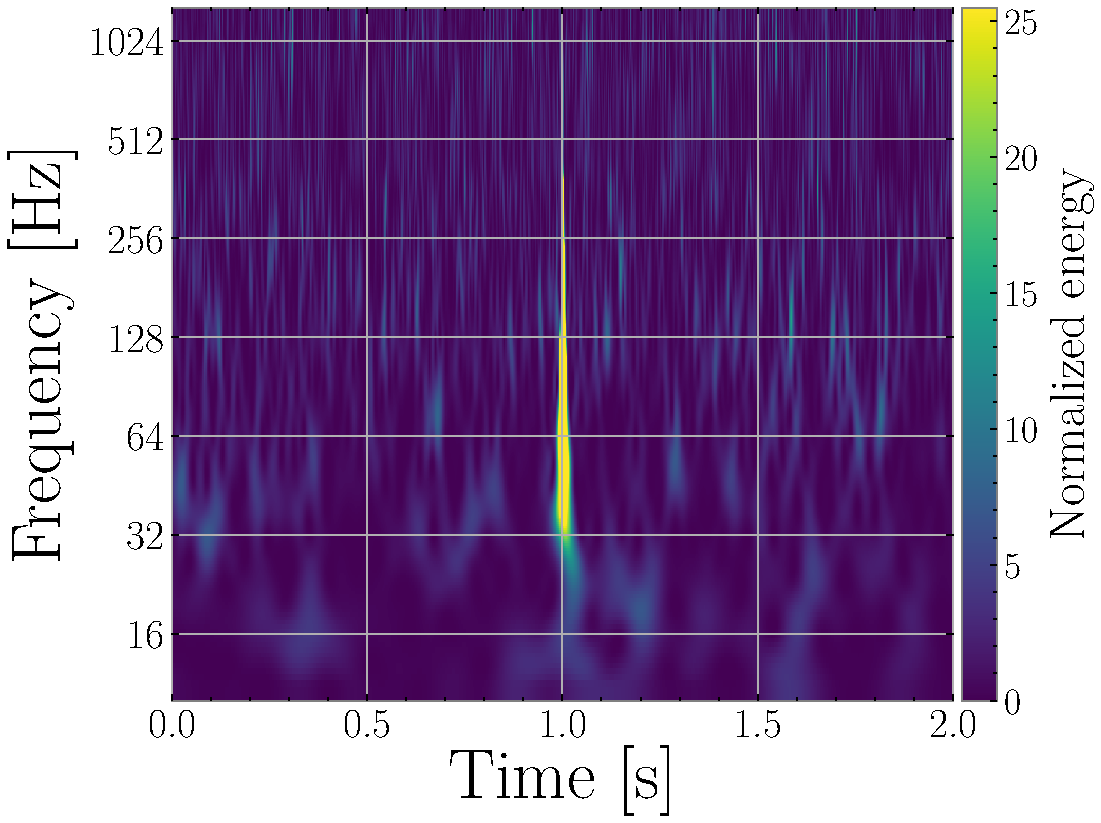
\includegraphics[width=\linewidth]{figures/gspy_input.pdf}
%   \caption{Input glitch}
%   \label{fig:de_gspy_input}
% \end{subfigure}
% \hspace{0.05\linewidth}
% \begin{subfigure}[t]{0.3\linewidth}
%   \centering
%   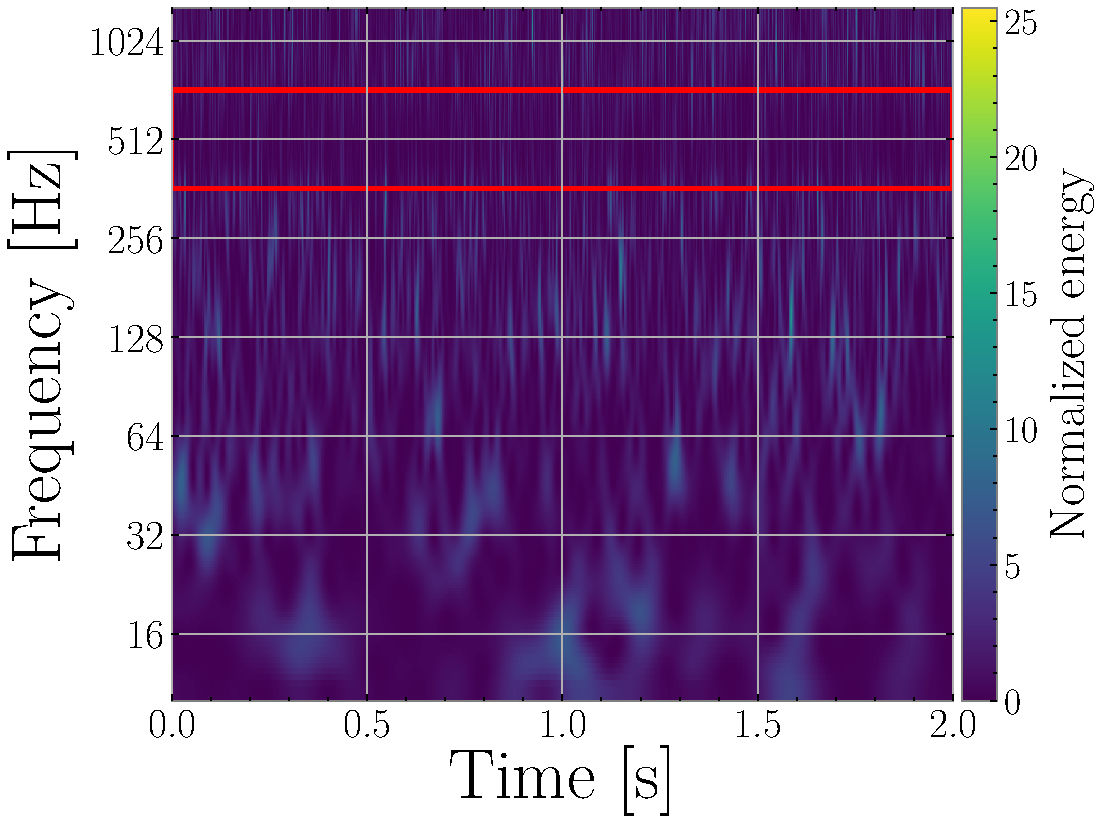
\includegraphics[width=\linewidth]{figures/gspy_output_no_tl.pdf}
%   \caption{No transfer learning}
%   \label{fig:de_gspy_output_no_tl}
% \end{subfigure}

% \vspace{0.8em}

% \begin{subfigure}[t]{0.3\linewidth}
%   \centering
%   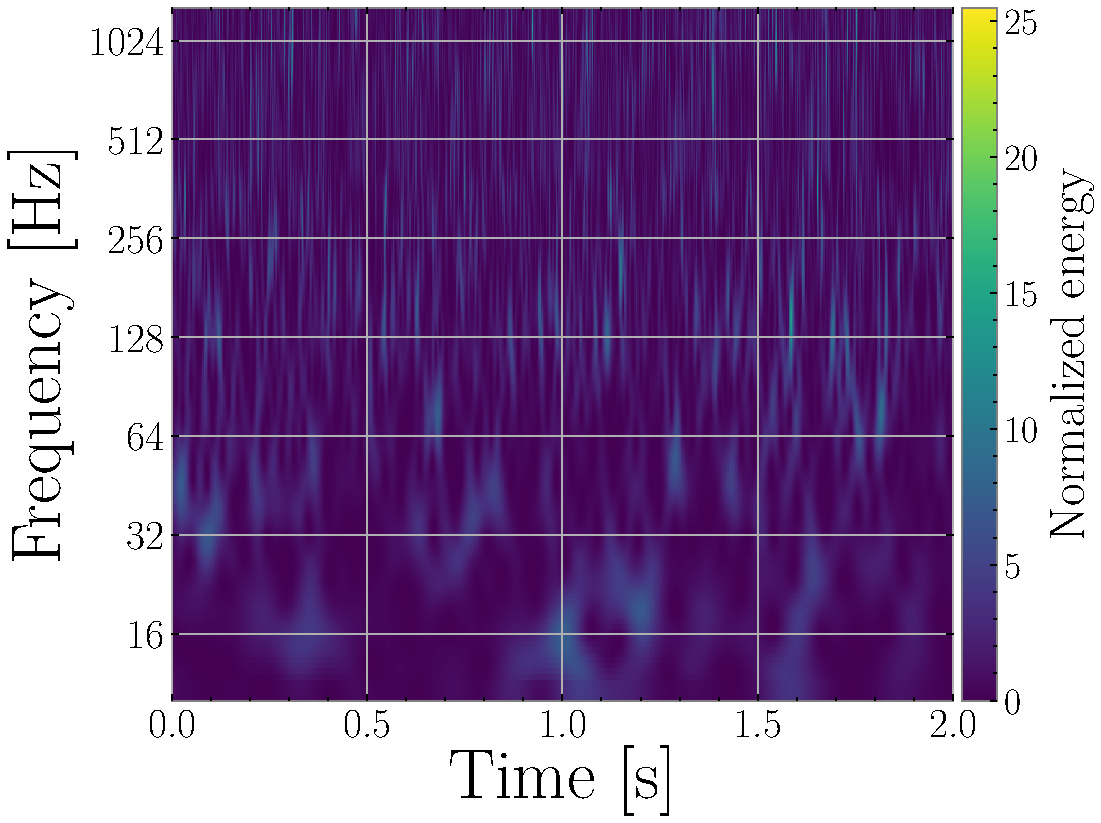
\includegraphics[width=\linewidth]{figures/gspy_output.pdf}
%   \caption{With transfer learning}
%   \label{fig:de_gspy_output}
% \end{subfigure}
% \hspace{0.05\linewidth}
% \begin{subfigure}[t]{0.3\linewidth}
%   \centering
%   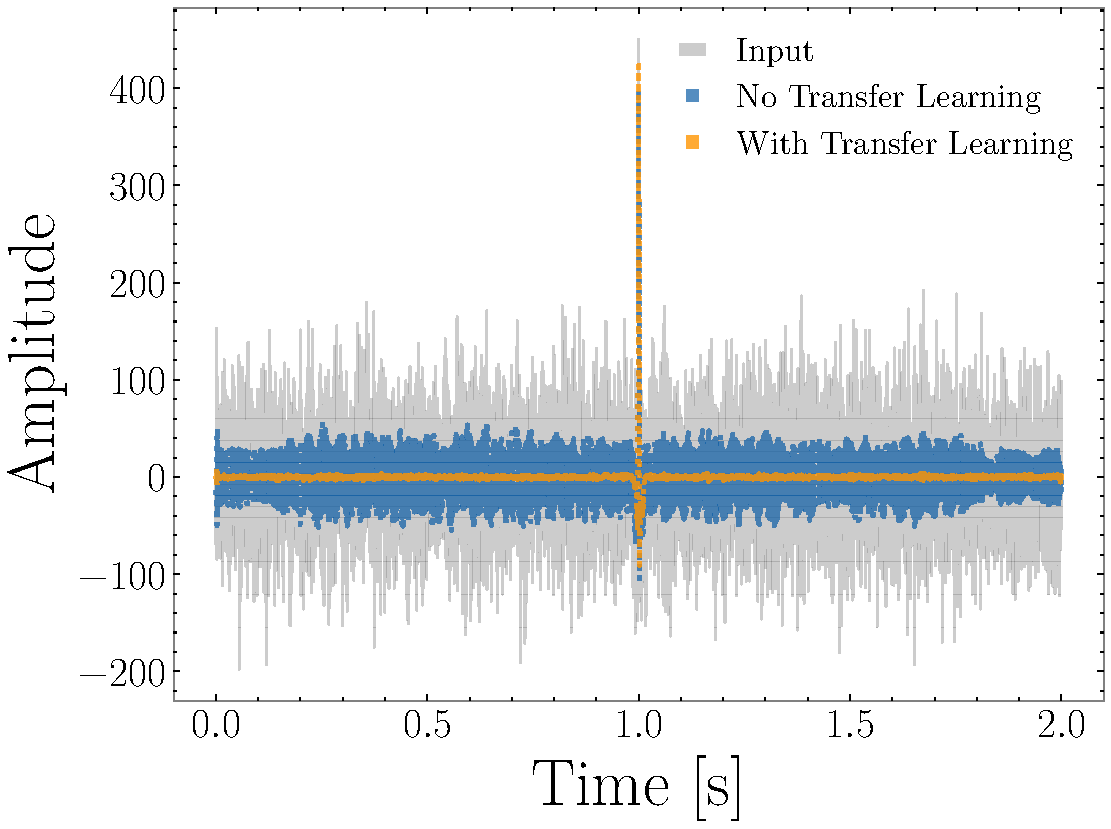
\includegraphics[width=\linewidth]{figures/gspy_ts.pdf}
%   \caption{Time-series outputs}
%   \label{fig:de_gspy_ts}
% \end{subfigure}

% \caption{Reconstruction of a Blip glitch from LIGO Hanford O3a with and without transfer learning. Without transfer learning (b), narrow line features at $512\,$Hz common in real LIGO noise are incorrectly subtracted. After fine-tuning on real detector noise (c), these features are preserved. The time-domain input and reconstructed waveforms are shown in (d).}
% \label{fig:de_gspy_transfer_learning}
% \end{figure}

% Figure~\ref{fig:de_gspy_examples} shows additional reconstruction examples for three distinct glitch classes.
% For most classes, the $Q$-scan residual after glitch subtraction closely resembles detector background noise, confirming effective glitch removal.

% \begin{figure}[ht]
% \centering
% 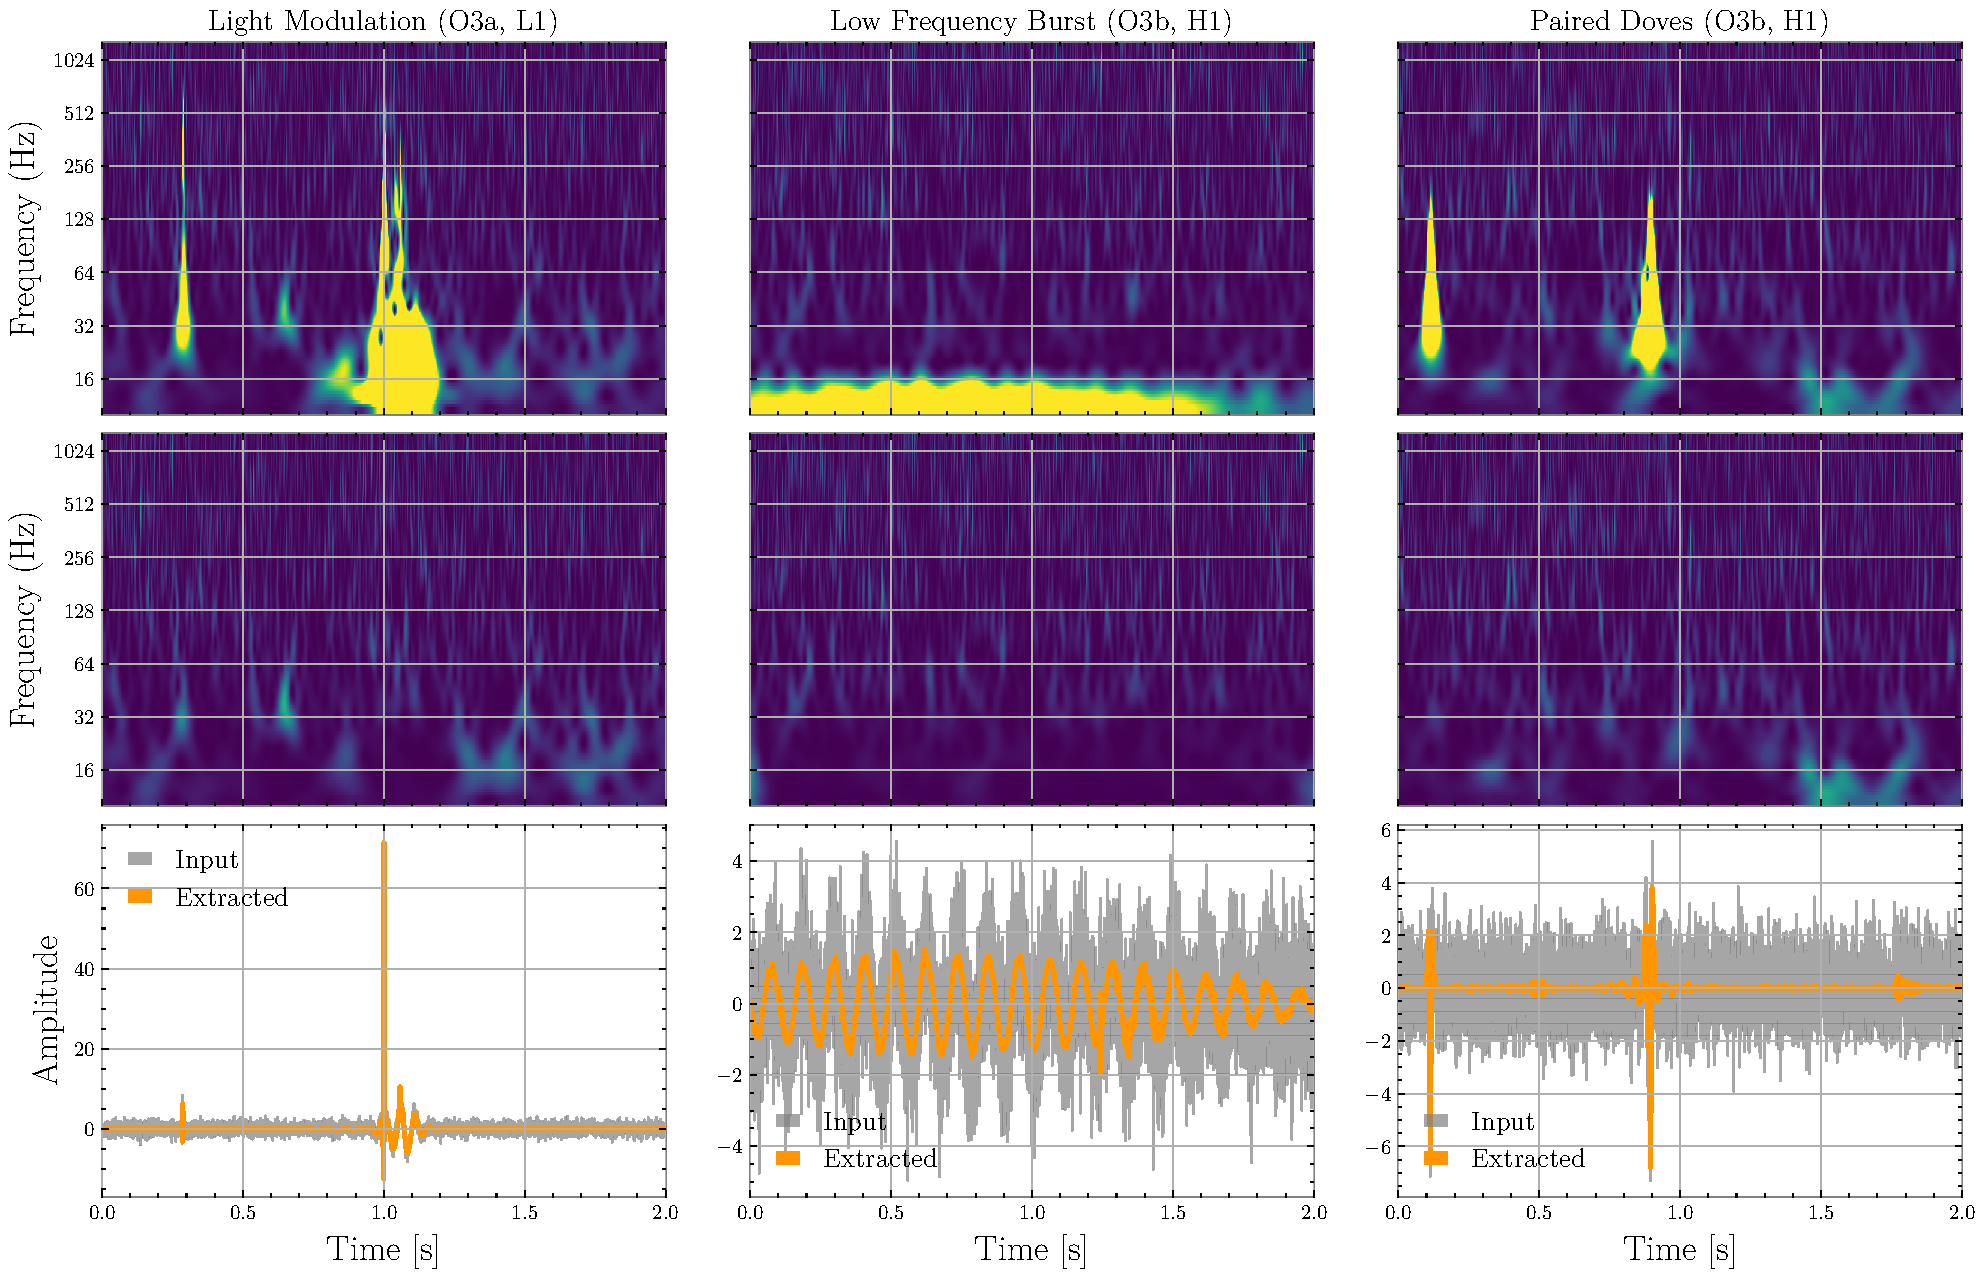
\includegraphics[width=0.99\linewidth]{figures/gspy_selected_examples_set_2.pdf}
% \caption{DeepExtractor reconstructions for three glitch classes: Light Modulation, Low Frequency Burst, and Paired Doves. The top row shows $Q$-scans of the input; the middle row shows $Q$-scans of the residual after glitch subtraction; the bottom row shows the corresponding time-domain waveforms.}
% \label{fig:de_gspy_examples}
% \end{figure}

\subsubsection{Classification evaluation using Gravity Spy}



To quantitatively assess reconstruction quality, we classify the 700 reconstructed glitches (100 per class) using the Gravity Spy classifier.
Tables~\ref{tab:de_summary} and~\ref{tab:de_per_class} summarize the results.
Of the 700 reconstructed glitches, 627 are correctly identified by Gravity Spy, corresponding to $\approx\!90\%$ overall accuracy.
Correctly classified reconstructions achieve a mean confidence of $96.77\%$, confirming that DeepExtractor effectively preserves the morphological characteristics recognized by Gravity Spy.
Misclassified samples show lower confidence ($84.84\%$), suggesting that classifier confidence may serve as a useful quality veto.

\begin{table}[h]
\centering
\caption{Summary of Gravity Spy results on DeepExtractor reconstructions (100 samples per class, 700 total).}
\label{tab:de_summary}
\begin{tabular}{l r}
\toprule
Total samples                  & 700       \\
Correct predictions            & 627       \\
Incorrect predictions          & 73        \\
\midrule
Overall accuracy               & 89.57\,\% \\
Mean confidence (correct)      & 96.77\,\% \\
Mean confidence (incorrect)    & 84.84\,\% \\
\bottomrule
\end{tabular}
\end{table}

\begin{table}[h]
\centering
\caption{Per-class correct prediction count and mean Gravity Spy confidence for DeepExtractor reconstructions.}
\label{tab:de_per_class}
\begin{tabular}{l r r}
\toprule
True label          & Correct count & Mean confidence (\%) \\
\midrule
Blip                & 100           & 99.30 \\
Fast Scattering     & 77            & 89.78 \\
Koi Fish            & 79            & 91.59 \\
Low Frequency Burst & 100           & 99.85 \\
Scattered Light     & 83            & 96.95 \\
Tomte               & 96            & 98.21 \\
Whistle             & 92            & 99.33 \\
\bottomrule
\end{tabular}
\end{table}

Table~\ref{tab:de_per_class} shows that class-level accuracy varies considerably.
All Blip and Low-Frequency Burst glitches are correctly classified, while Fast Scattering and Koi Fish achieve the lowest accuracies at 77\% and 79\%, respectively.
Figure~\ref{fig:de_confusion} shows the full confusion matrix.
Most misclassifications occur between morphologically similar classes: among the 21 misclassified Koi Fish glitches, 14 were labelled as Extremely Loud, consistent with their exceptionally high SNRs (220--1270) overwhelming finer morphological cues.
The 23 misclassified Fast Scattering samples are distributed across several related classes (Scattered Light, Tomte, Repeating Blips), reflecting the known morphological similarity between low-frequency scattering noise types.
Overall, the misclassification patterns are morphologically explainable and do not indicate systematic failure of the reconstruction.


\subsubsection{Unsupervised clustering with t-SNE and UMAP}

Figure~\ref{fig:de_3d_embeddings} shows three-dimensional t-SNE (left) and UMAP (right) embeddings of the DeepExtractor reconstructions, visualized from three complementary viewpoints.
The reconstructions form well-separated clusters that align closely with the Gravity Spy labels, demonstrating that morphologically distinct glitch types occupy distinct regions of the time-domain latent space.
Partial overlap between the Blip and Koi Fish clusters is visible, consistent with prior observations that these classes may share a physical origin~\citep{Areeda2017}.
The good clustering structure validates that the 31,511 DeepExtractor reconstructions used to train GlitchGAN are morphologically representative of the seven glitch classes and are not dominated by reconstruction artifacts or label noise.

\begin{figure*}[tp]
\centering
\begin{subfigure}{0.45\textwidth}
    \centering
    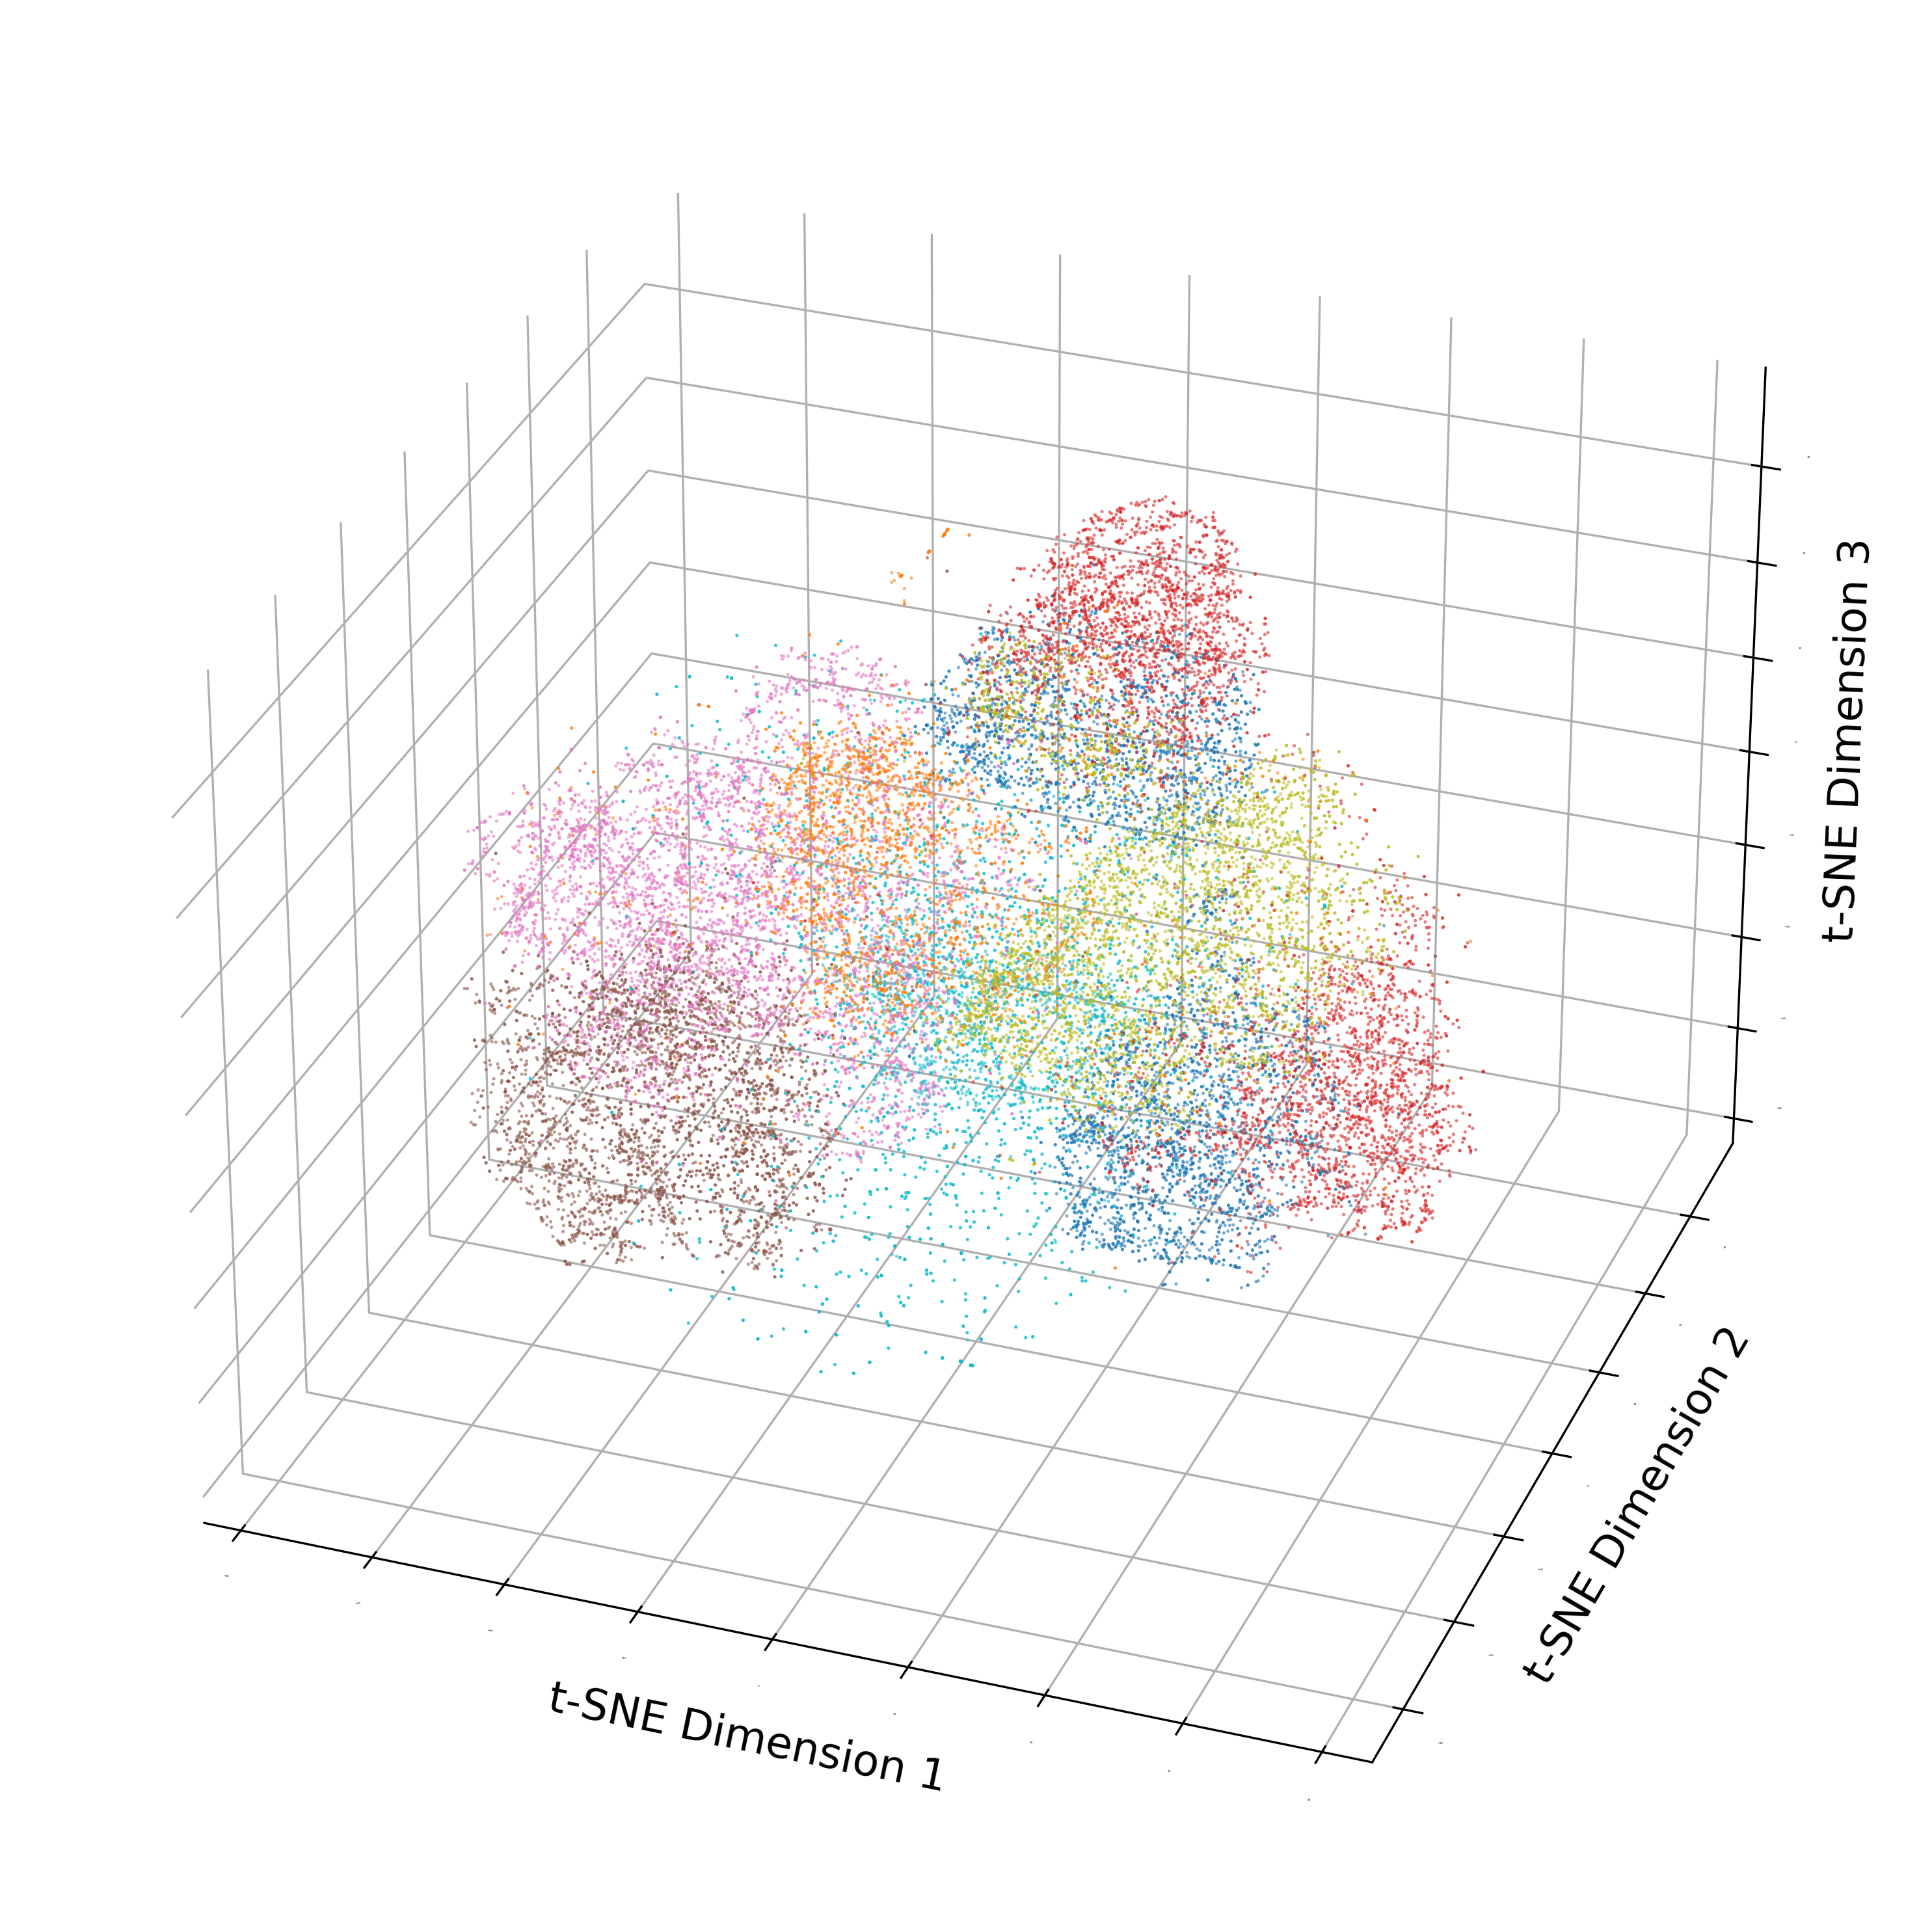
\includegraphics[width=\linewidth,keepaspectratio]{figures/tsne_3d_view_improved_standard_view.png}
\end{subfigure}\hfill
\begin{subfigure}{0.45\textwidth}
    \centering
    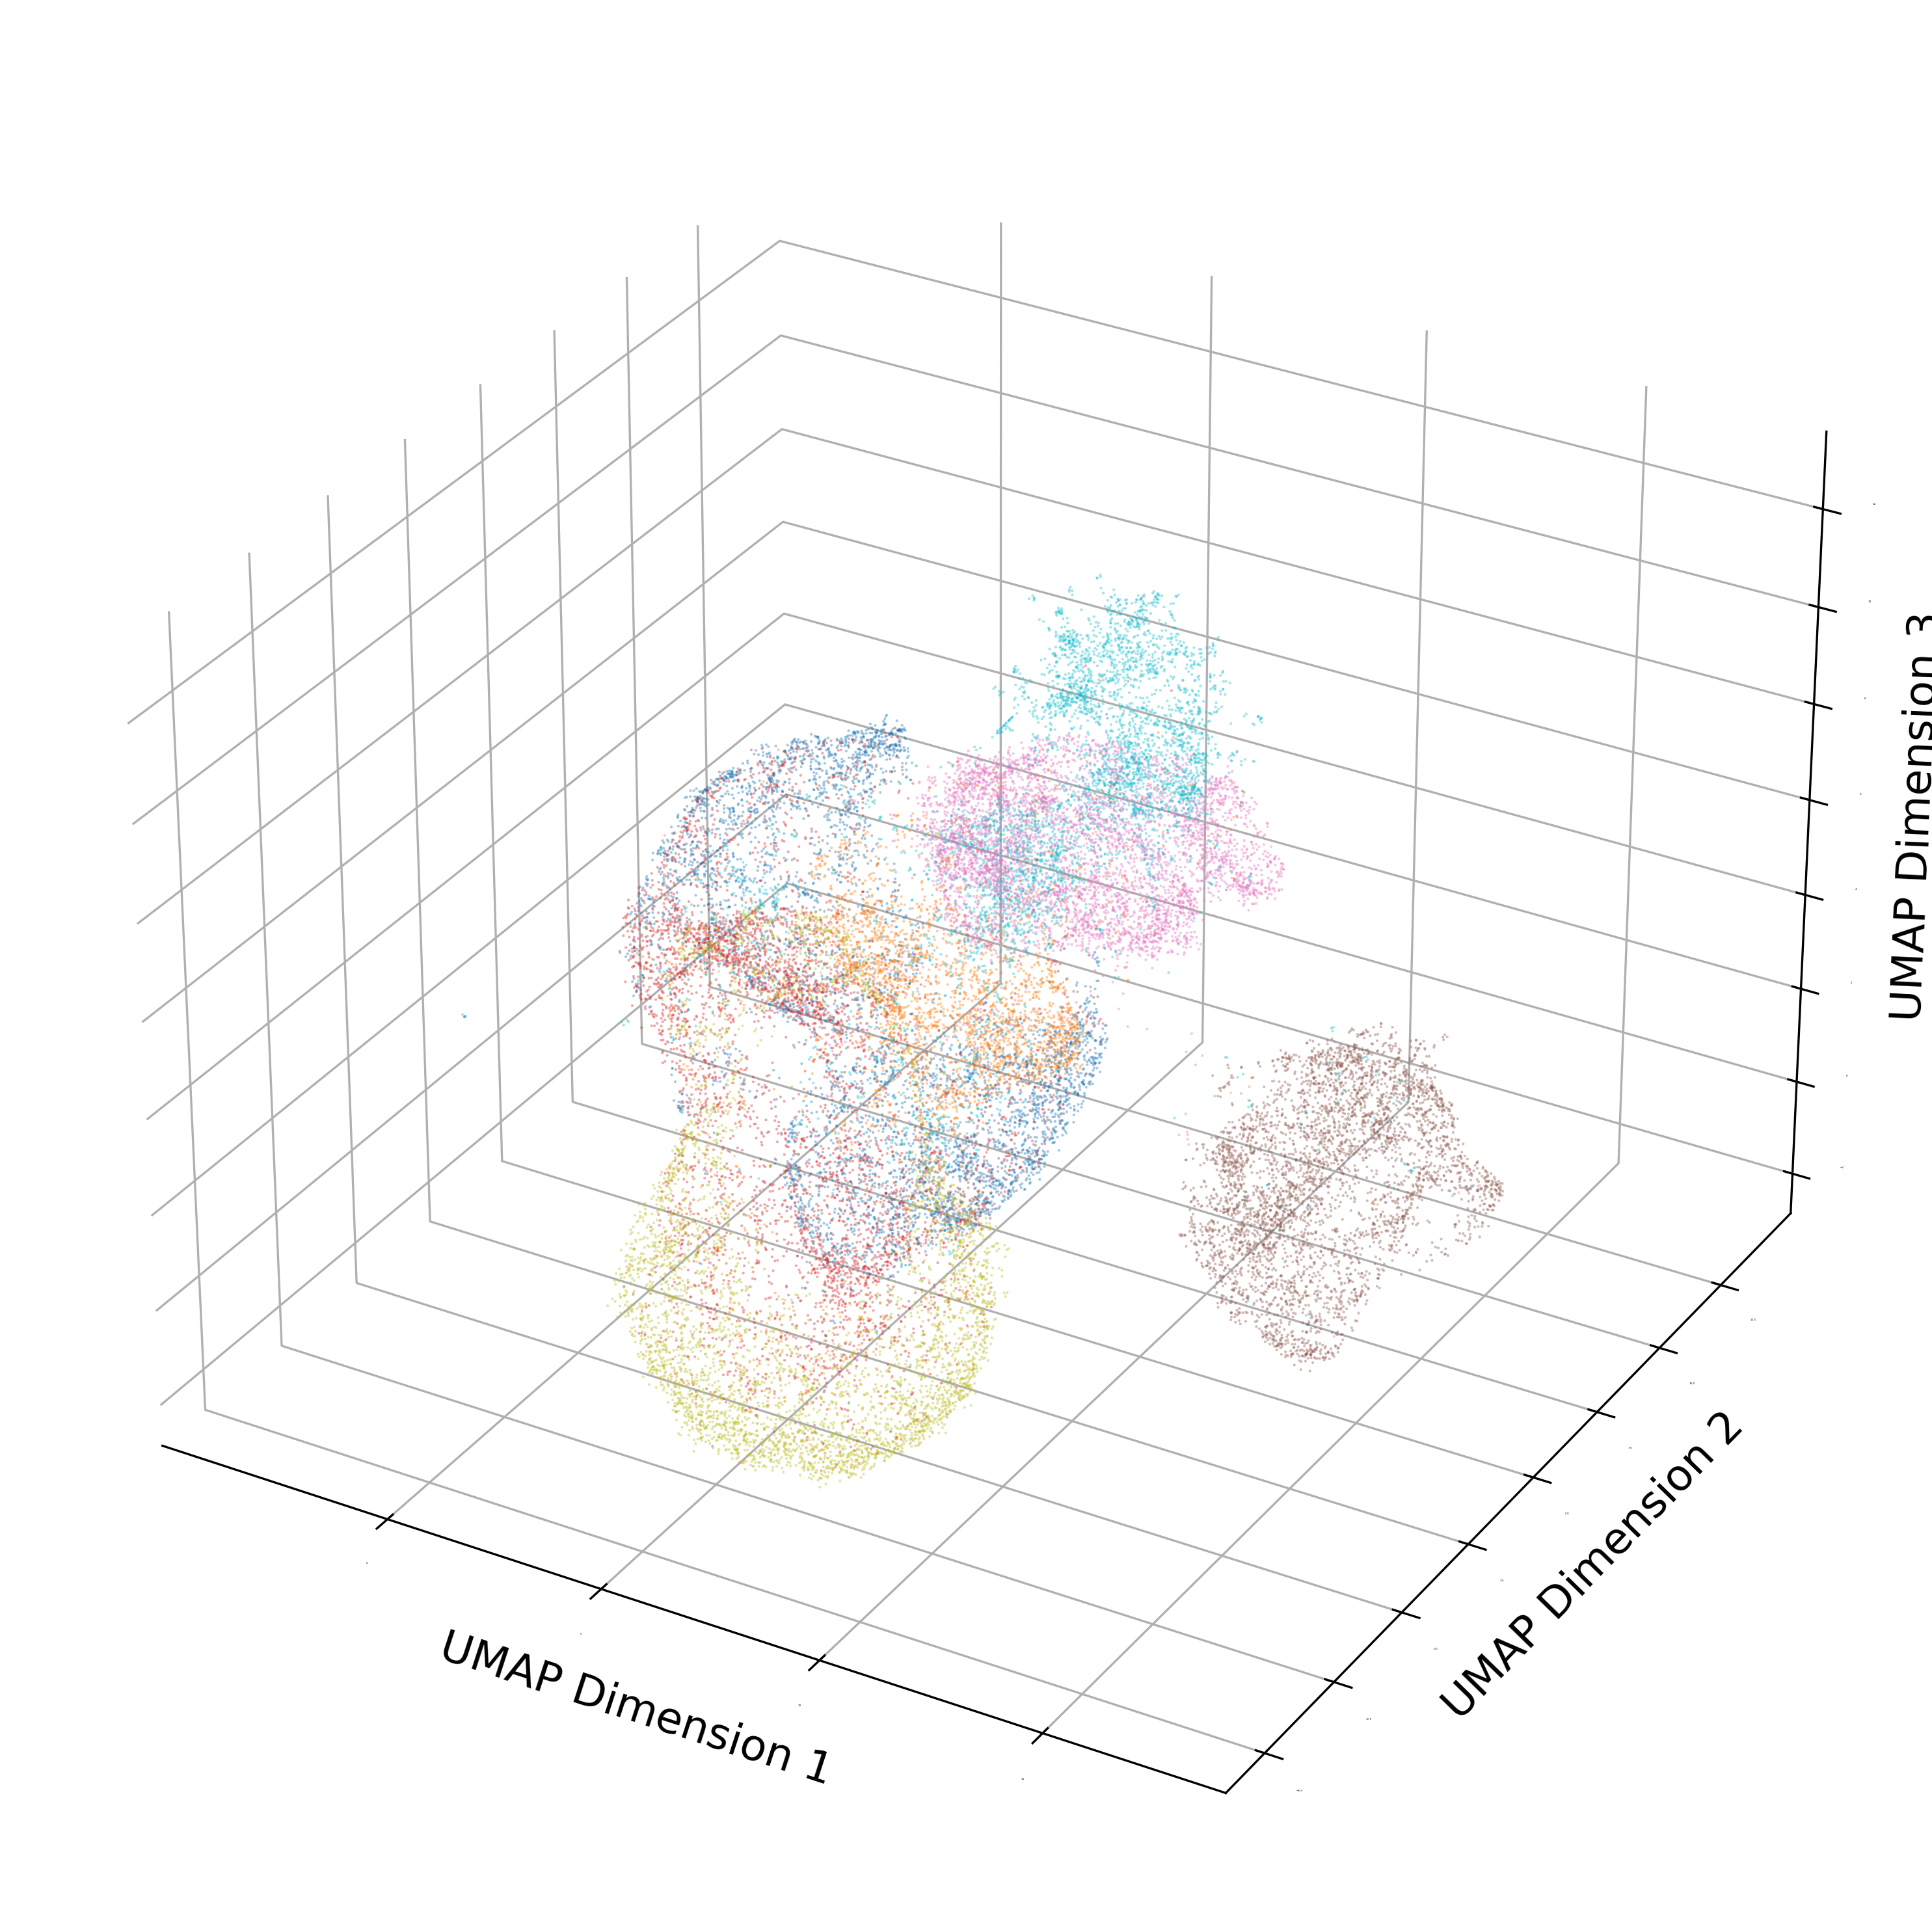
\includegraphics[width=\linewidth,keepaspectratio]{figures/umap_3d_view_improved_standard_view.png}
\end{subfigure}
\vspace{-1em}
\begin{subfigure}{0.45\textwidth}
    \hspace*{-1cm}
    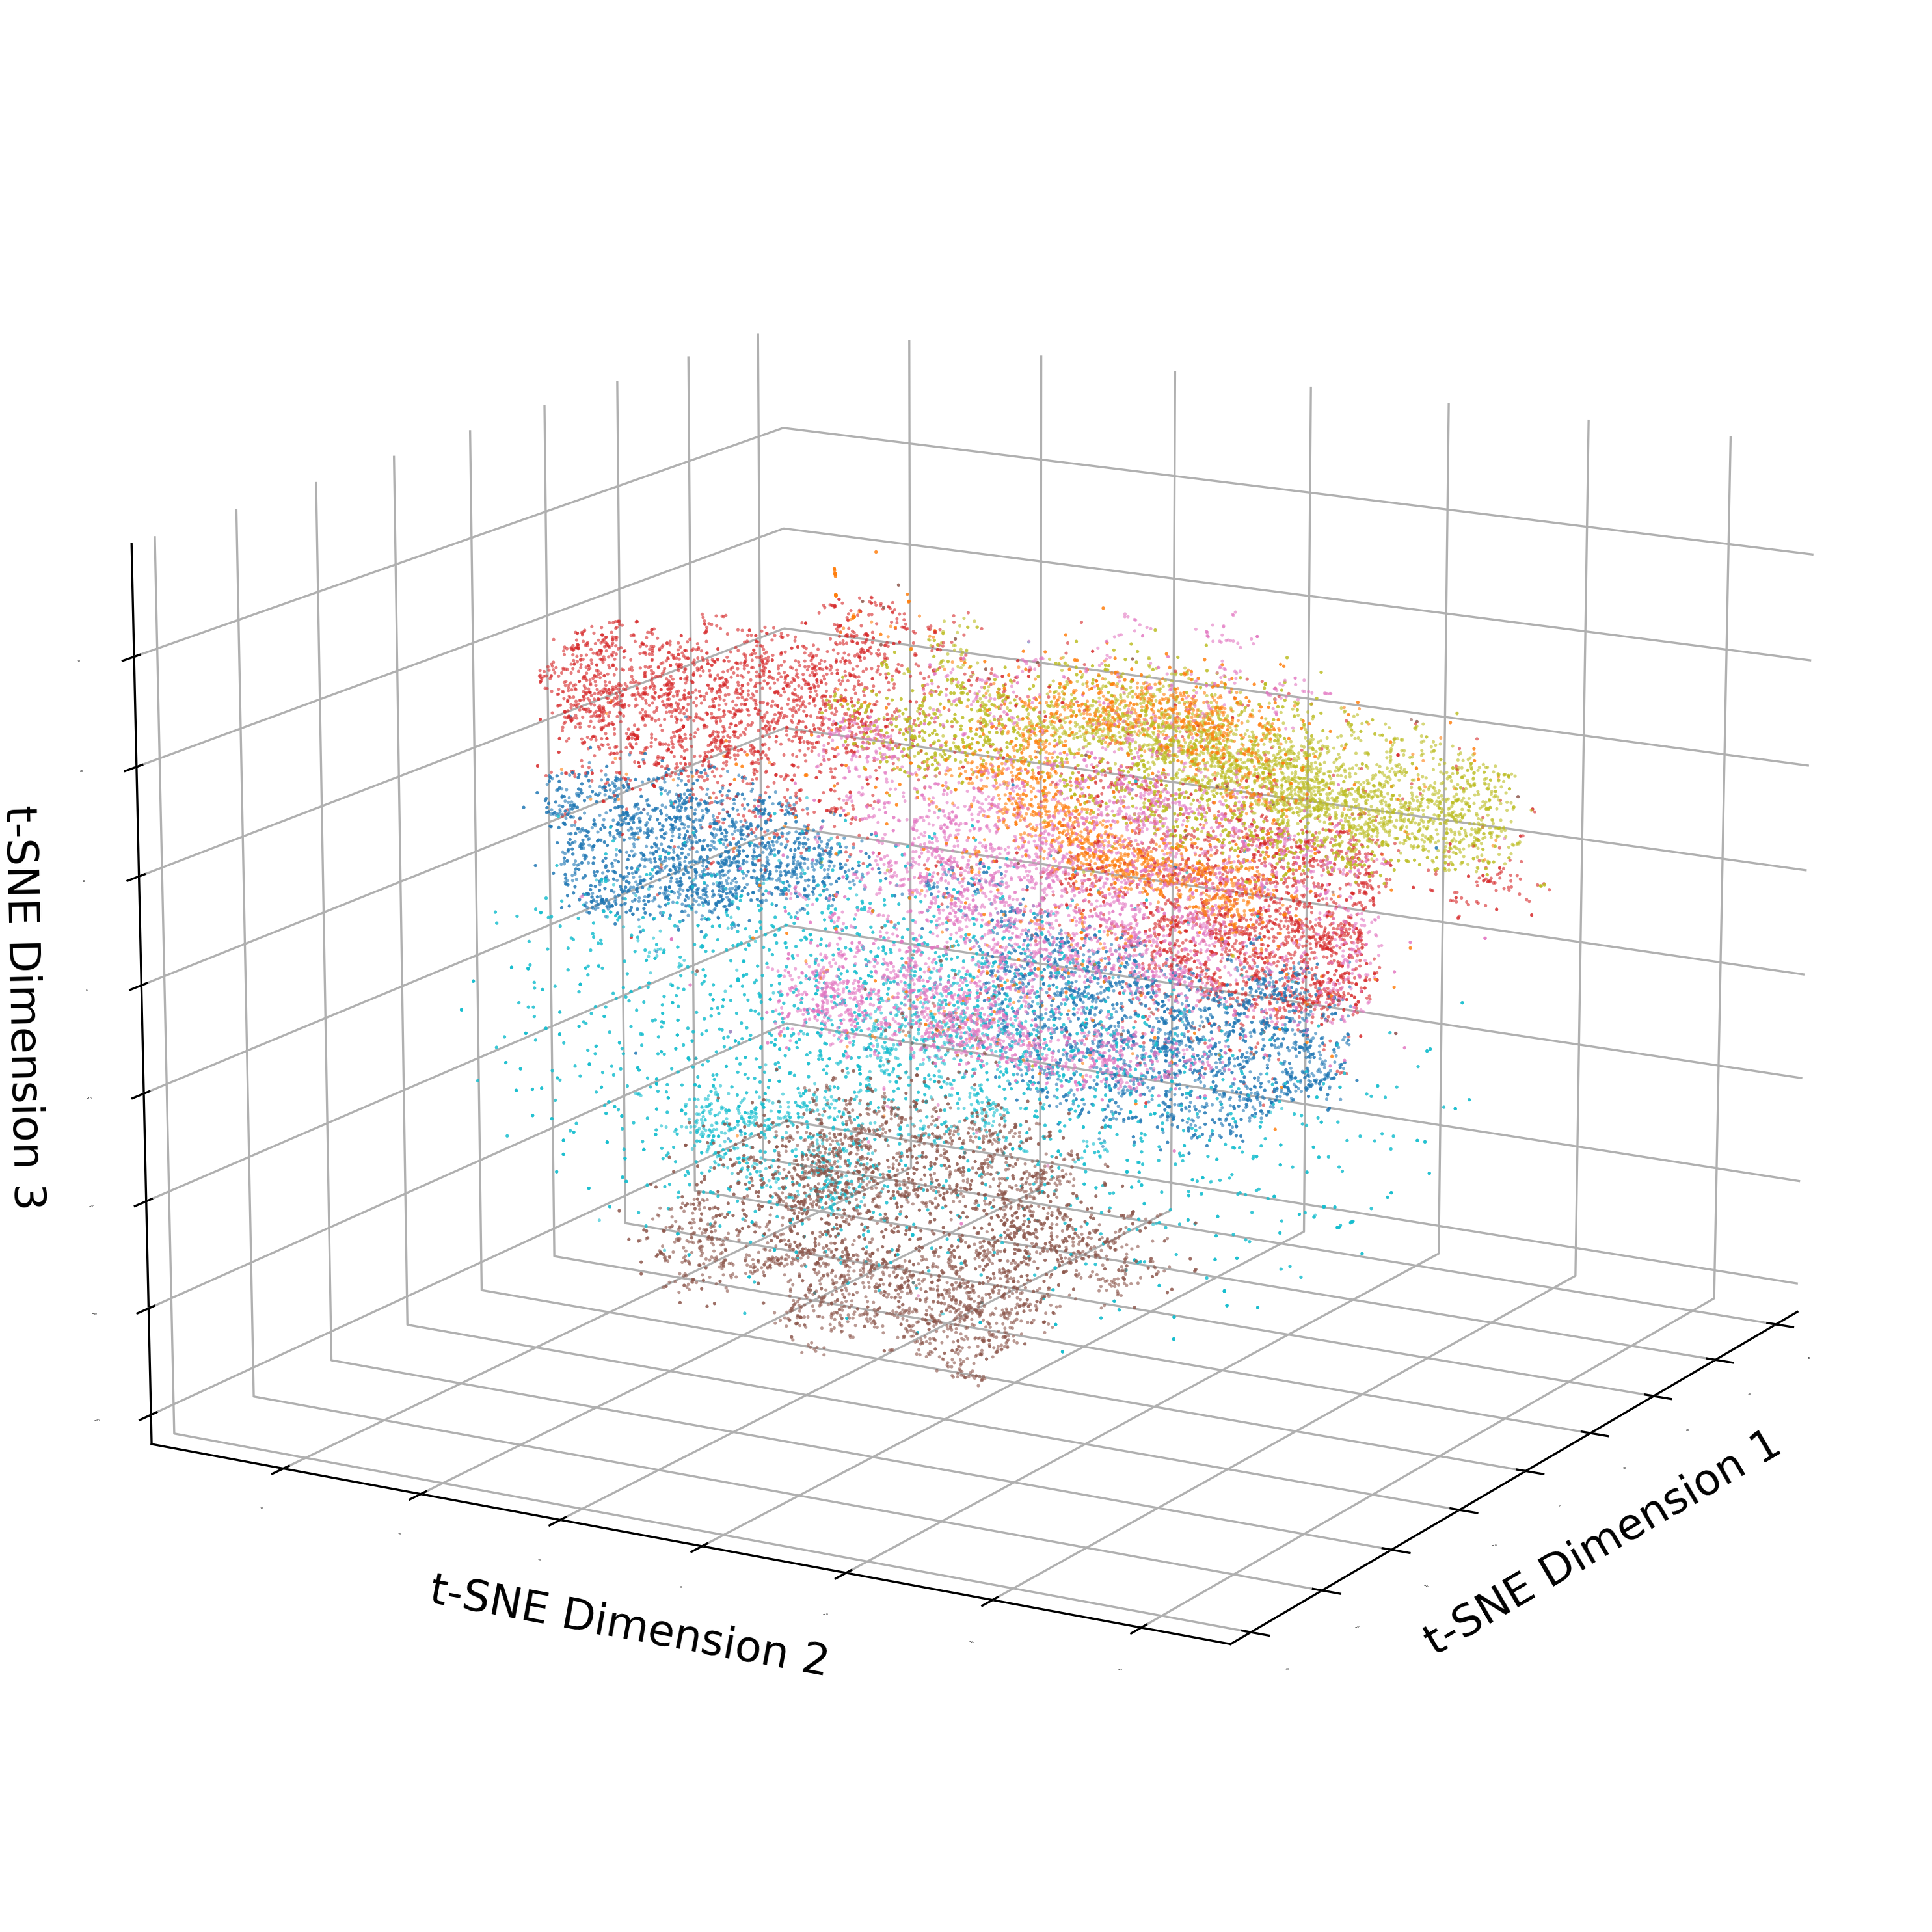
\includegraphics[width=\linewidth,keepaspectratio]{figures/tsne_3d_view_improved_angled_front_view.png}
\end{subfigure}\hfill
\begin{subfigure}{0.10\textwidth}
    \hspace*{-1cm}
    \raisebox{2cm}[0pt][0pt]{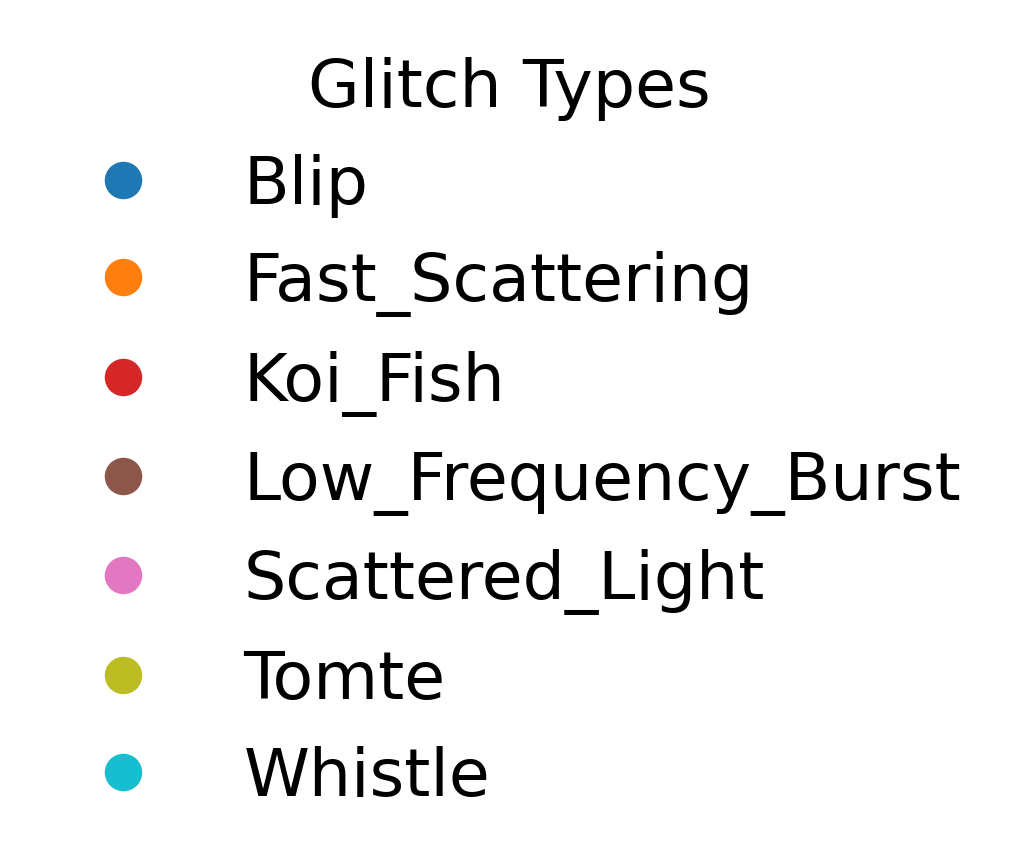
\includegraphics[width=2\linewidth,keepaspectratio]{figures/umap_3d_legend.png}}
\end{subfigure}\hfill
\begin{subfigure}{0.45\textwidth}
    \hspace*{1cm}
    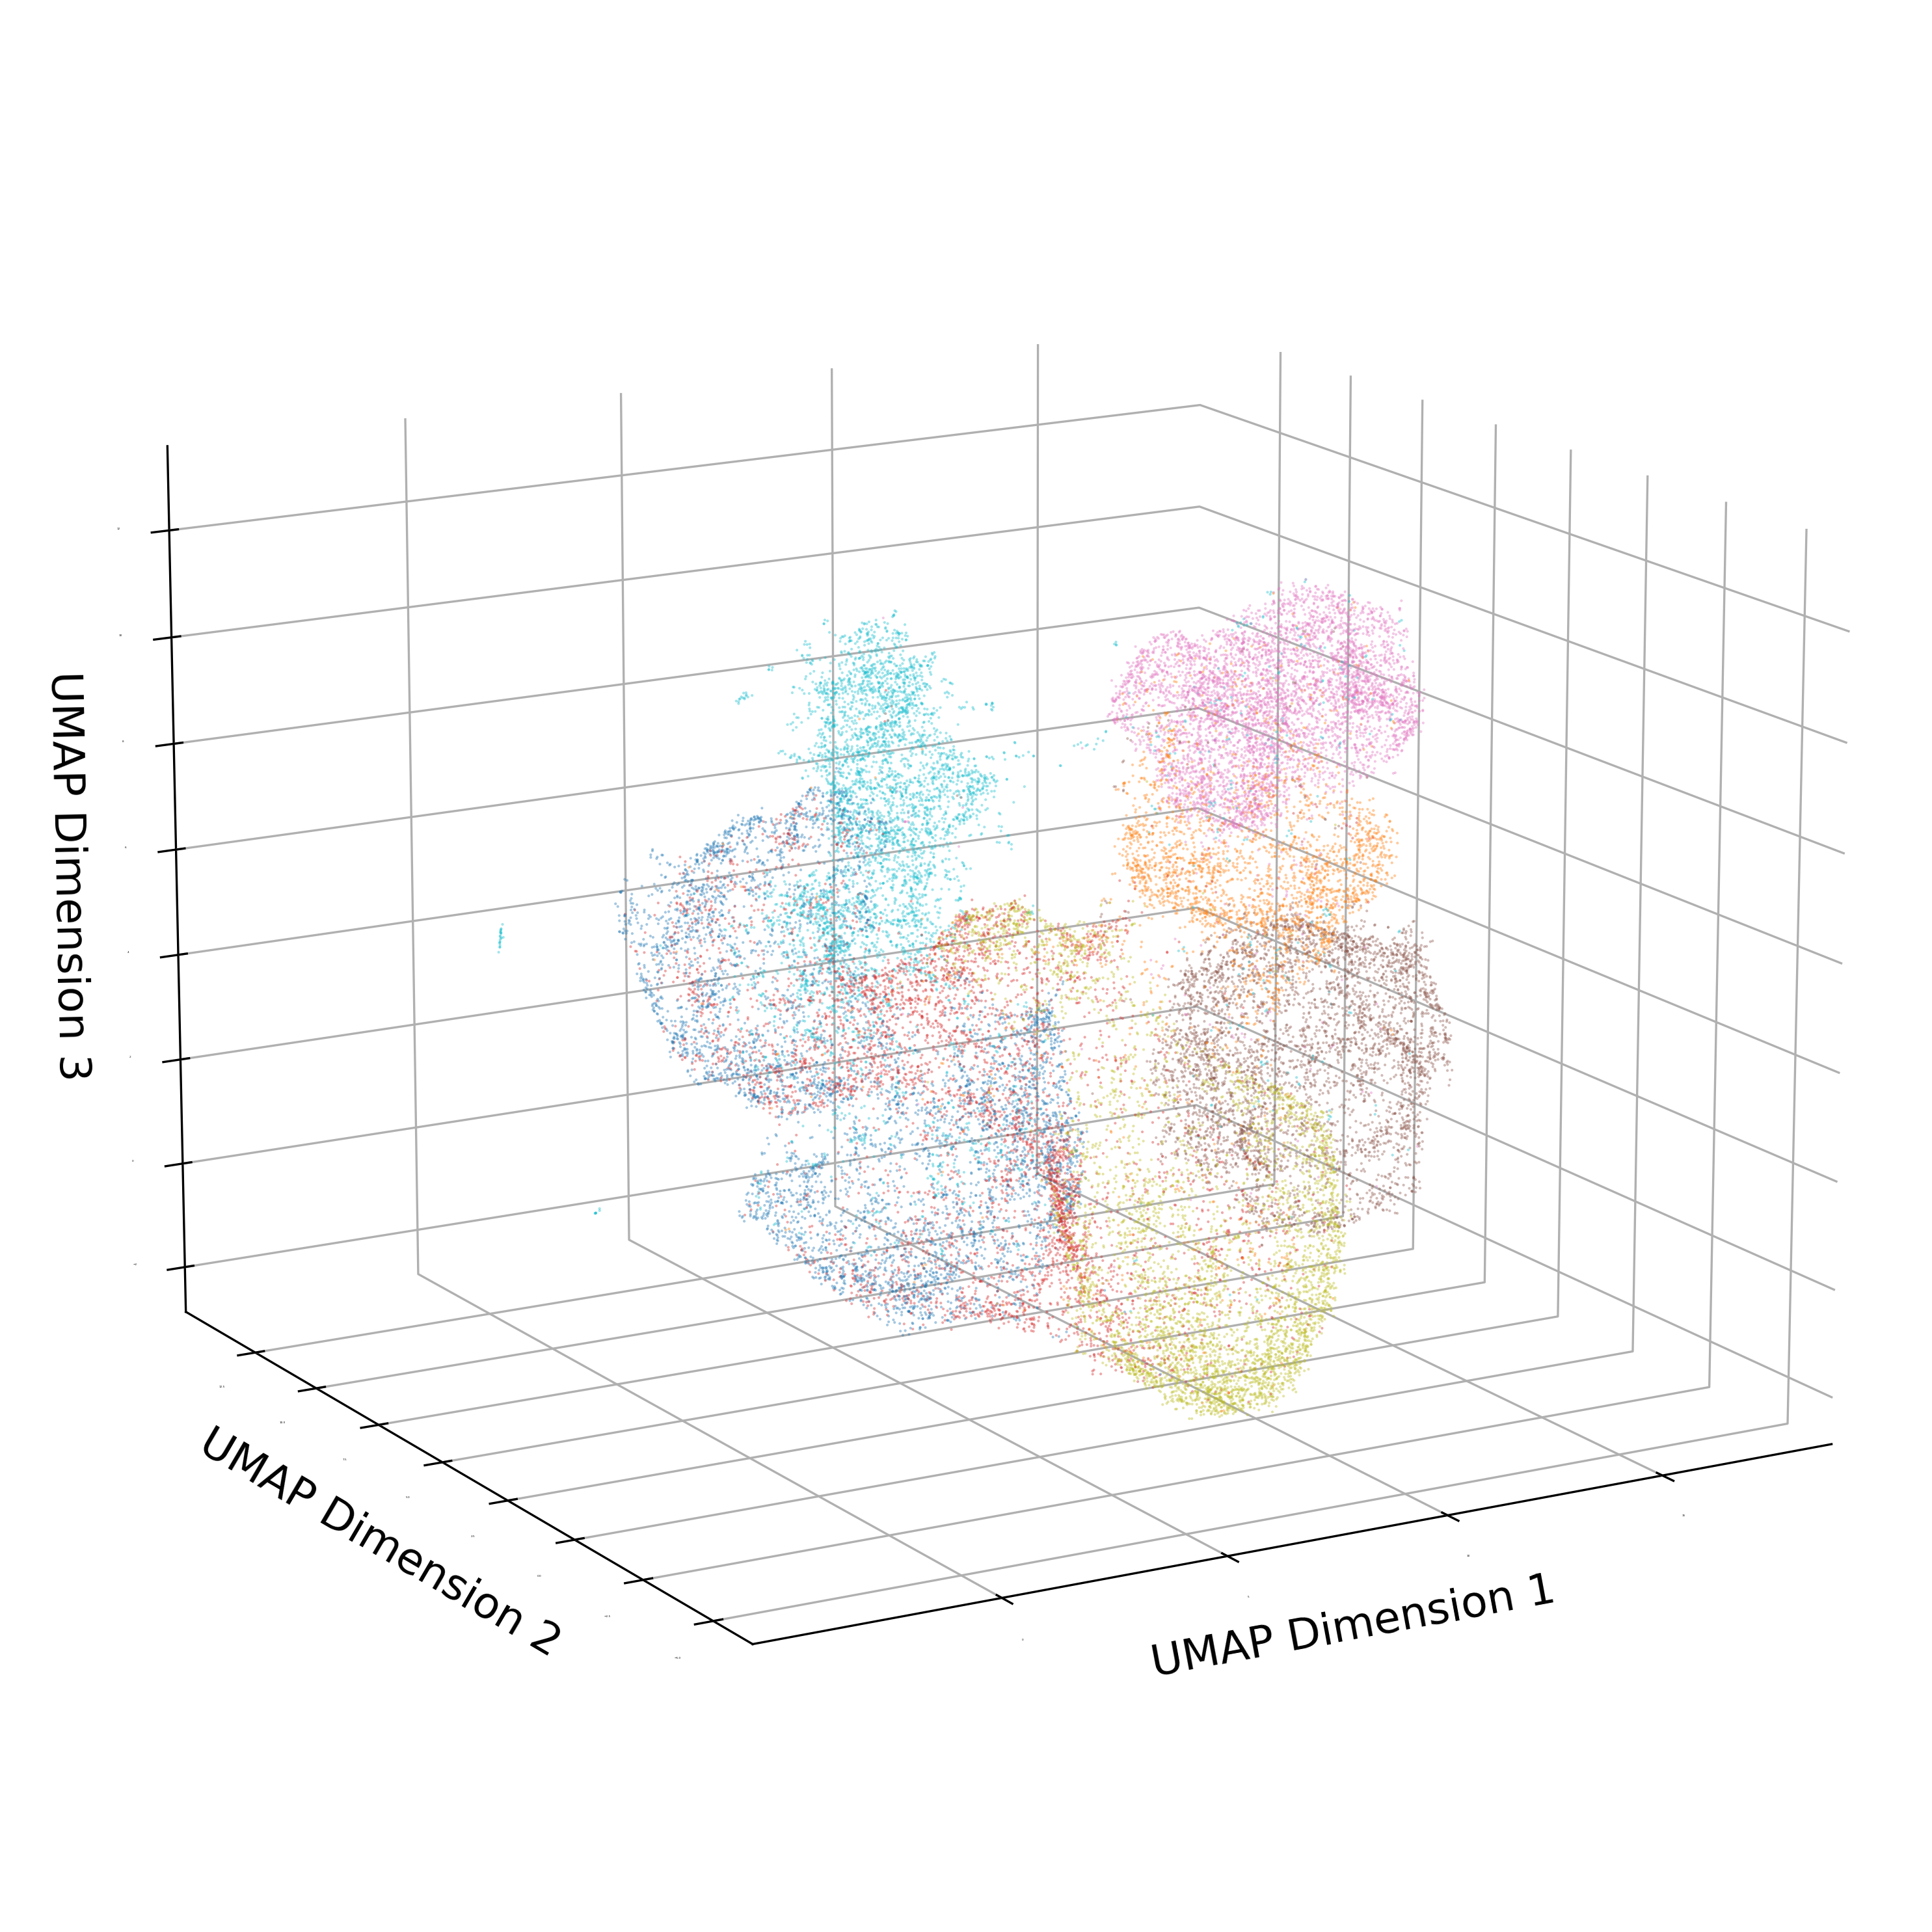
\includegraphics[width=\linewidth,keepaspectratio]{figures/umap_3d_view_improved_angled_front_view.png}
\end{subfigure}
\vspace{-1em}
\begin{subfigure}{0.45\textwidth}
    \centering
    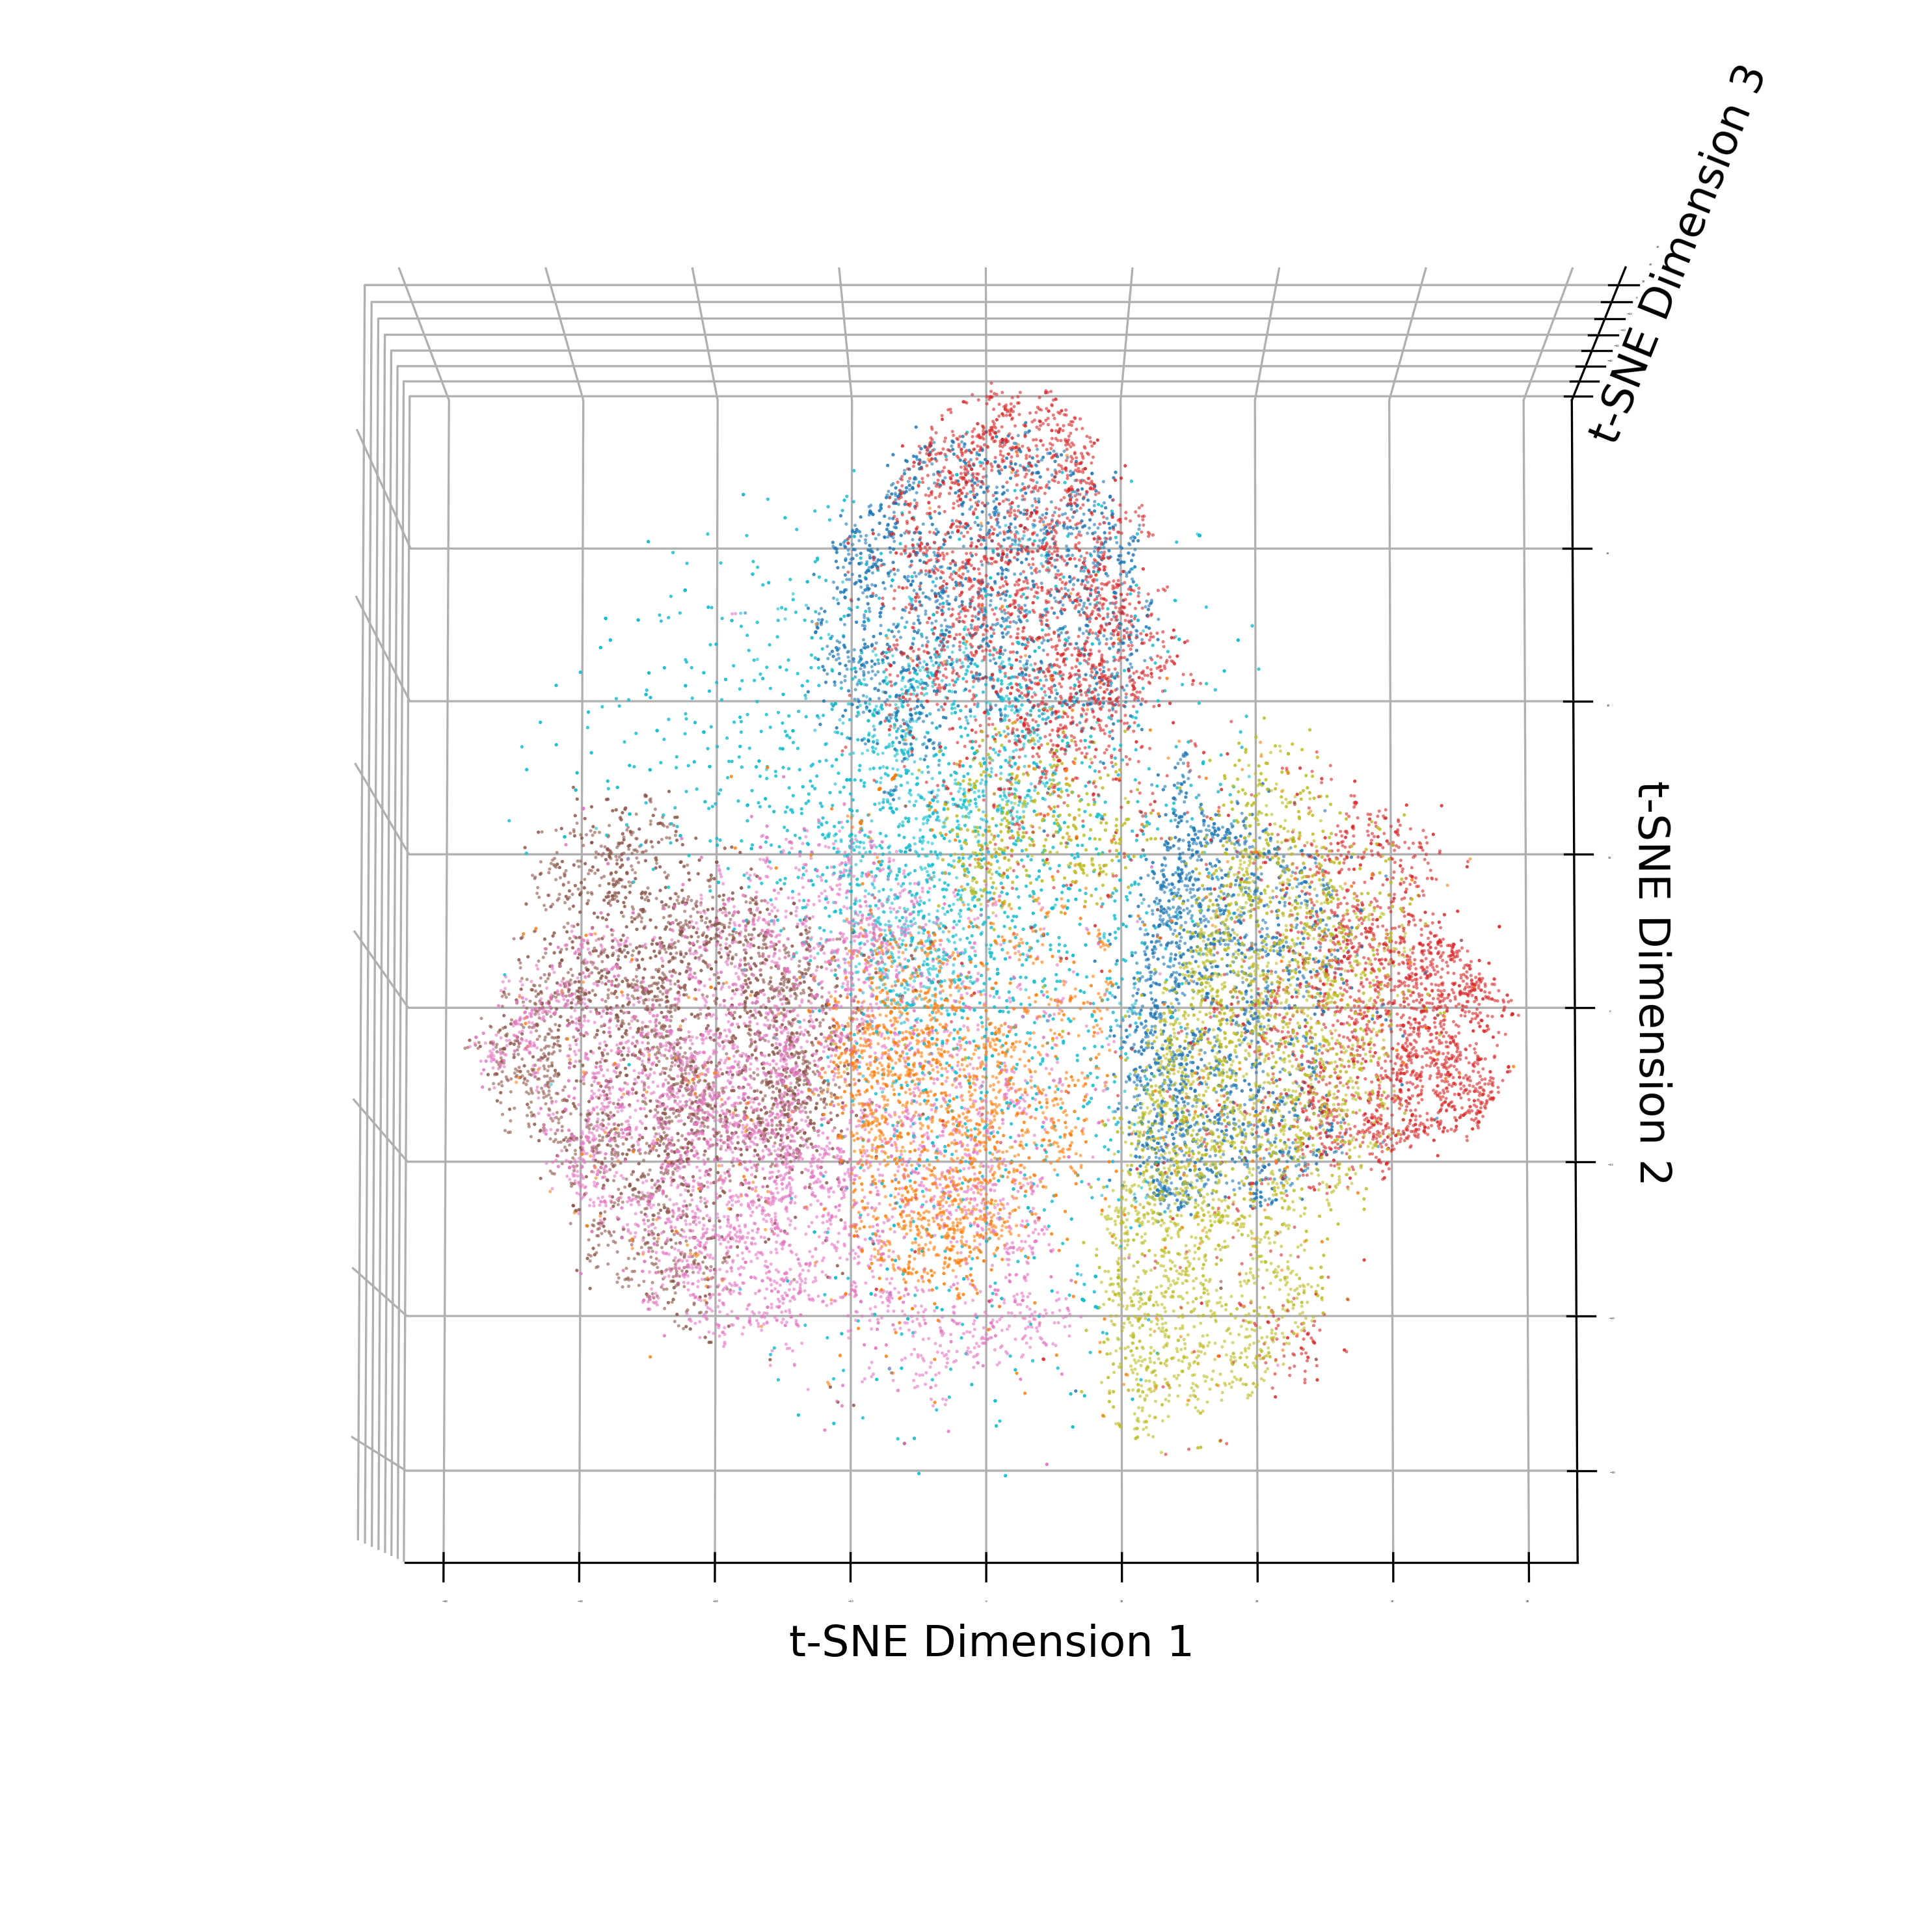
\includegraphics[width=\linewidth,keepaspectratio]{figures/tsne_3d_view_improved_near_top_down_view.png}
\end{subfigure}\hfill
\begin{subfigure}{0.45\textwidth}
    \centering
    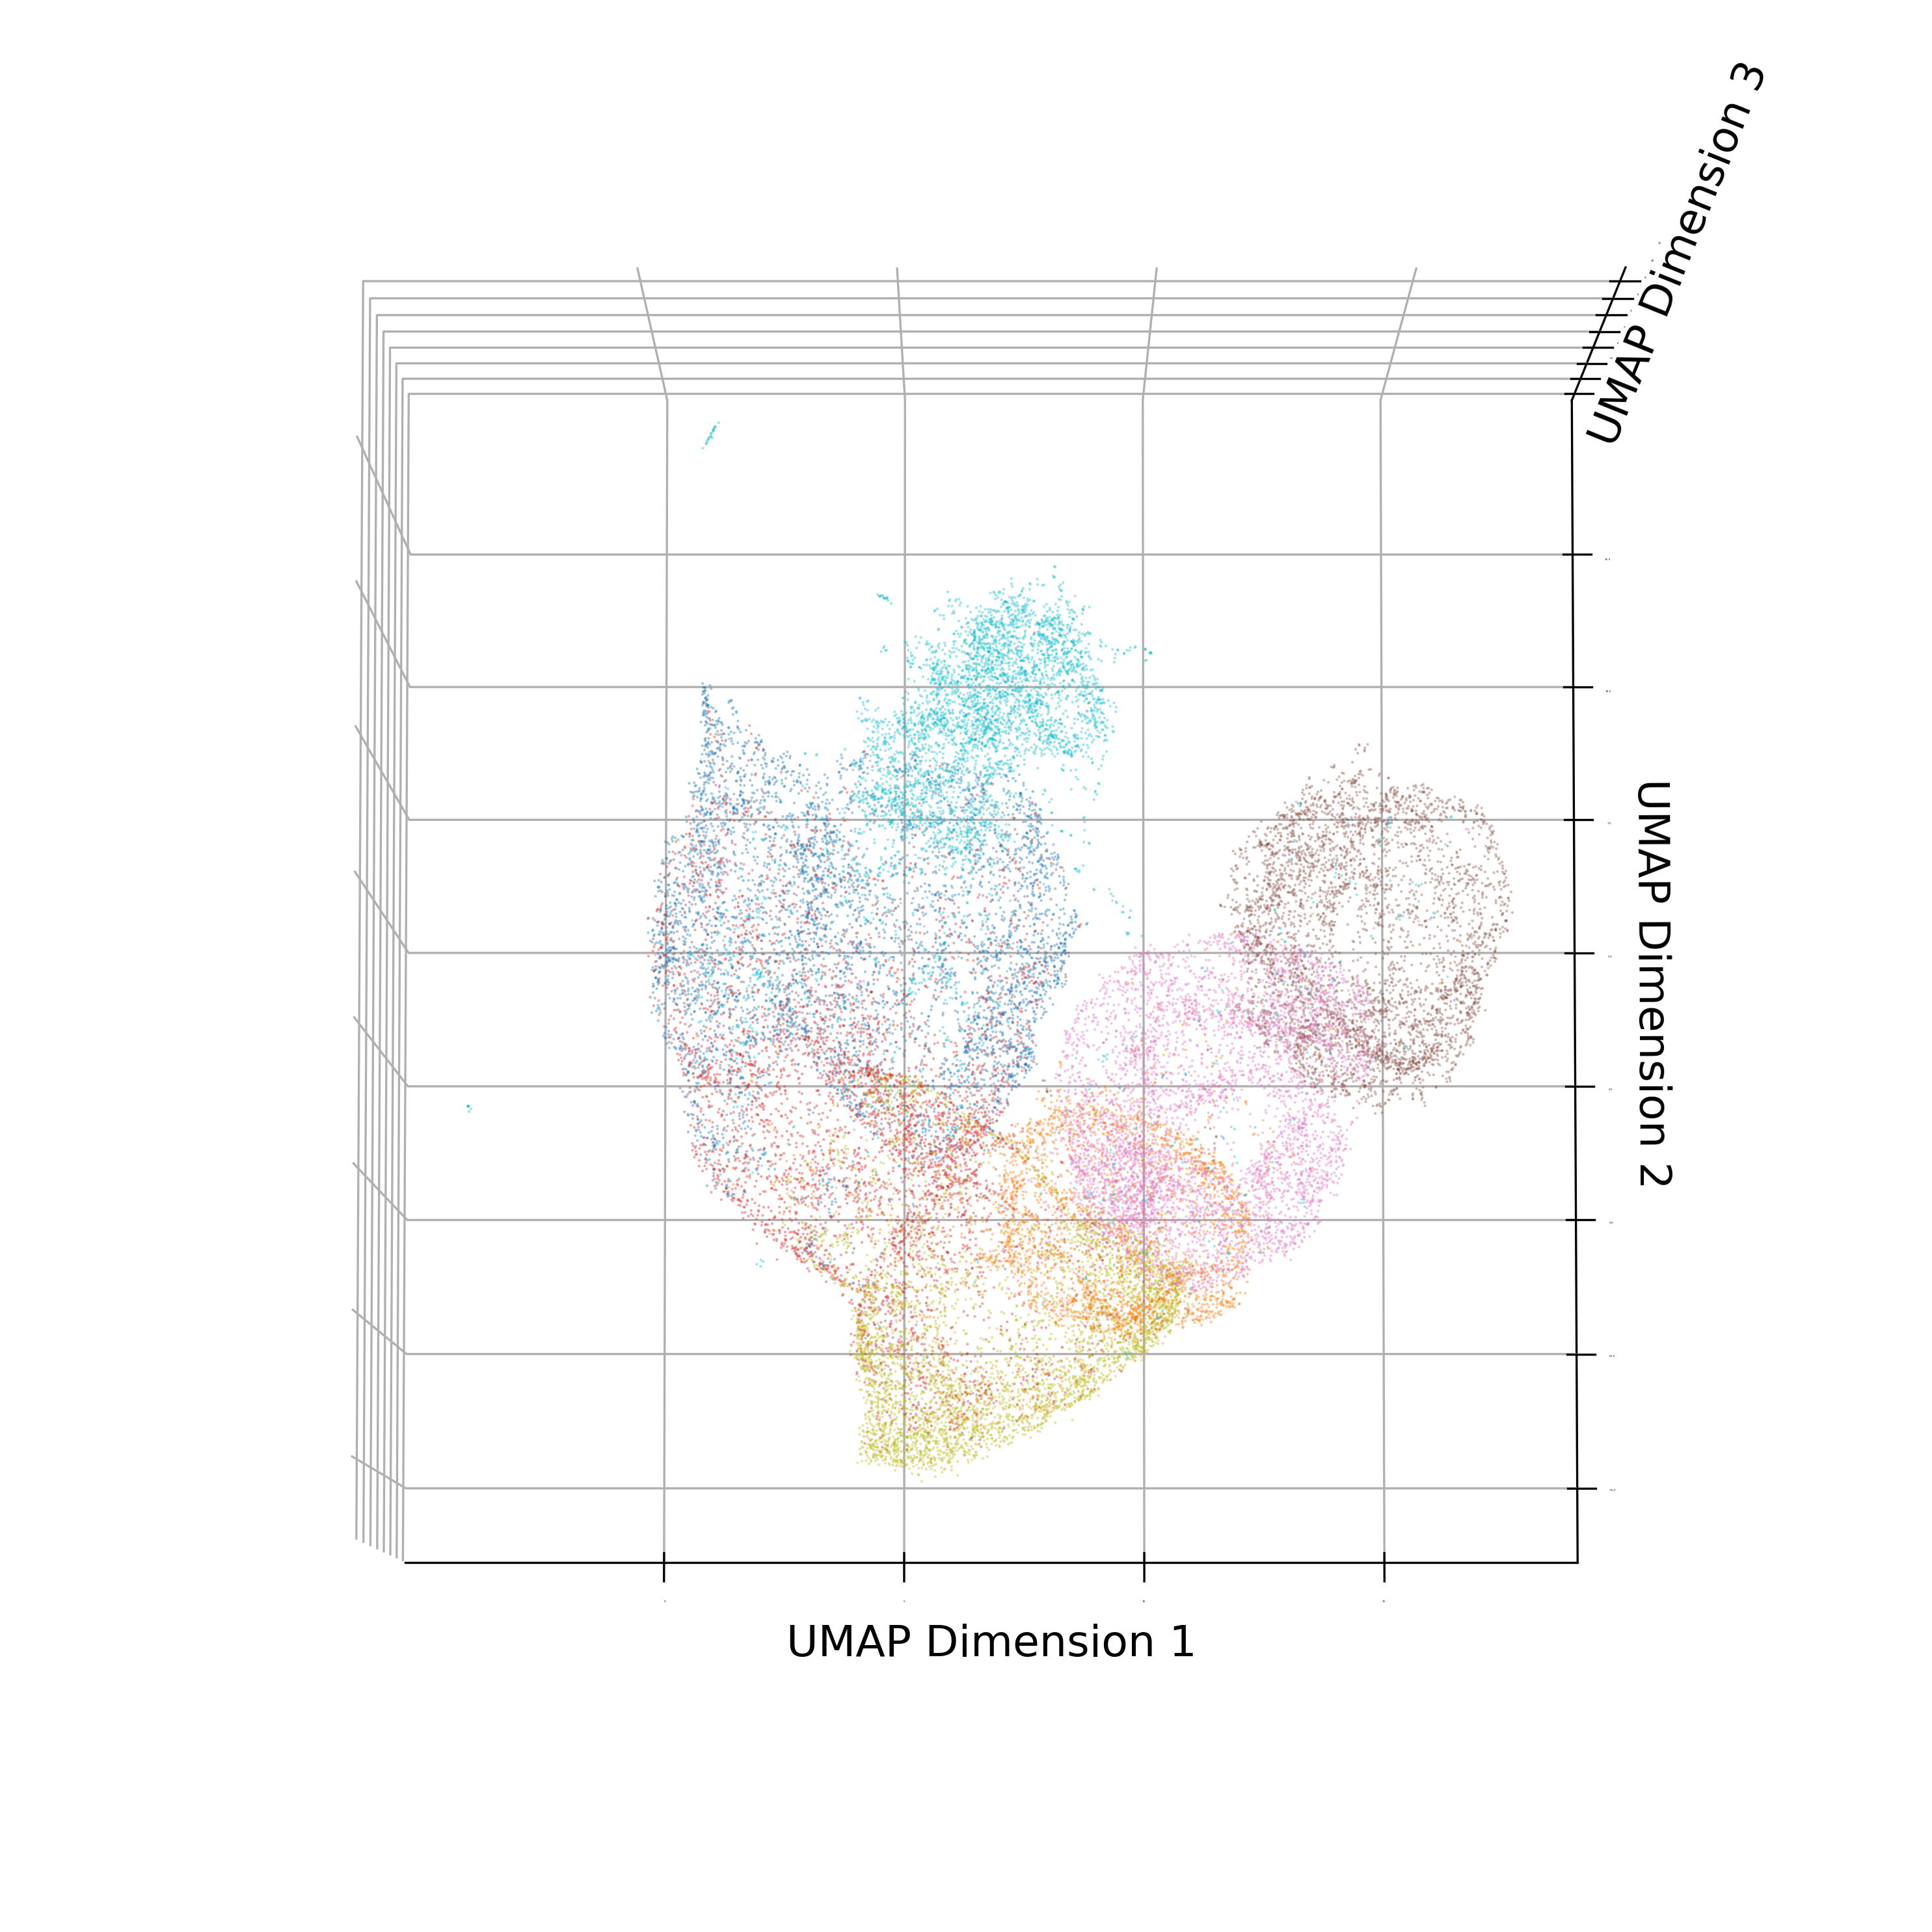
\includegraphics[width=\linewidth,keepaspectratio]{figures/umap_3d_view_improved_near_top_down_view.png}
\end{subfigure}
\caption{Three-dimensional t-SNE (left) and UMAP (right) embeddings of DeepExtractor reconstructions across three viewpoints. Colors correspond to Gravity Spy glitch classes. Well-separated clusters demonstrate that reconstructions preserve class-specific morphological structure in the time domain. The partial overlap between Blip and Koi Fish (visible in the middle row) is consistent with their known morphological proximity.}
\label{fig:de_3d_embeddings}
\end{figure*}

\subsection{Validation against Gravity Spy classifier}

To quantify synthetic glitch realism in a regime relevant to gravitational-wave data analysis, we injected generated glitches into quiet LIGO Hanford O3 background noise at SNR = 50 and classified them using the Gravity Spy classifier.
One hundred samples were generated per class.

\begin{figure*}[t]
\centering
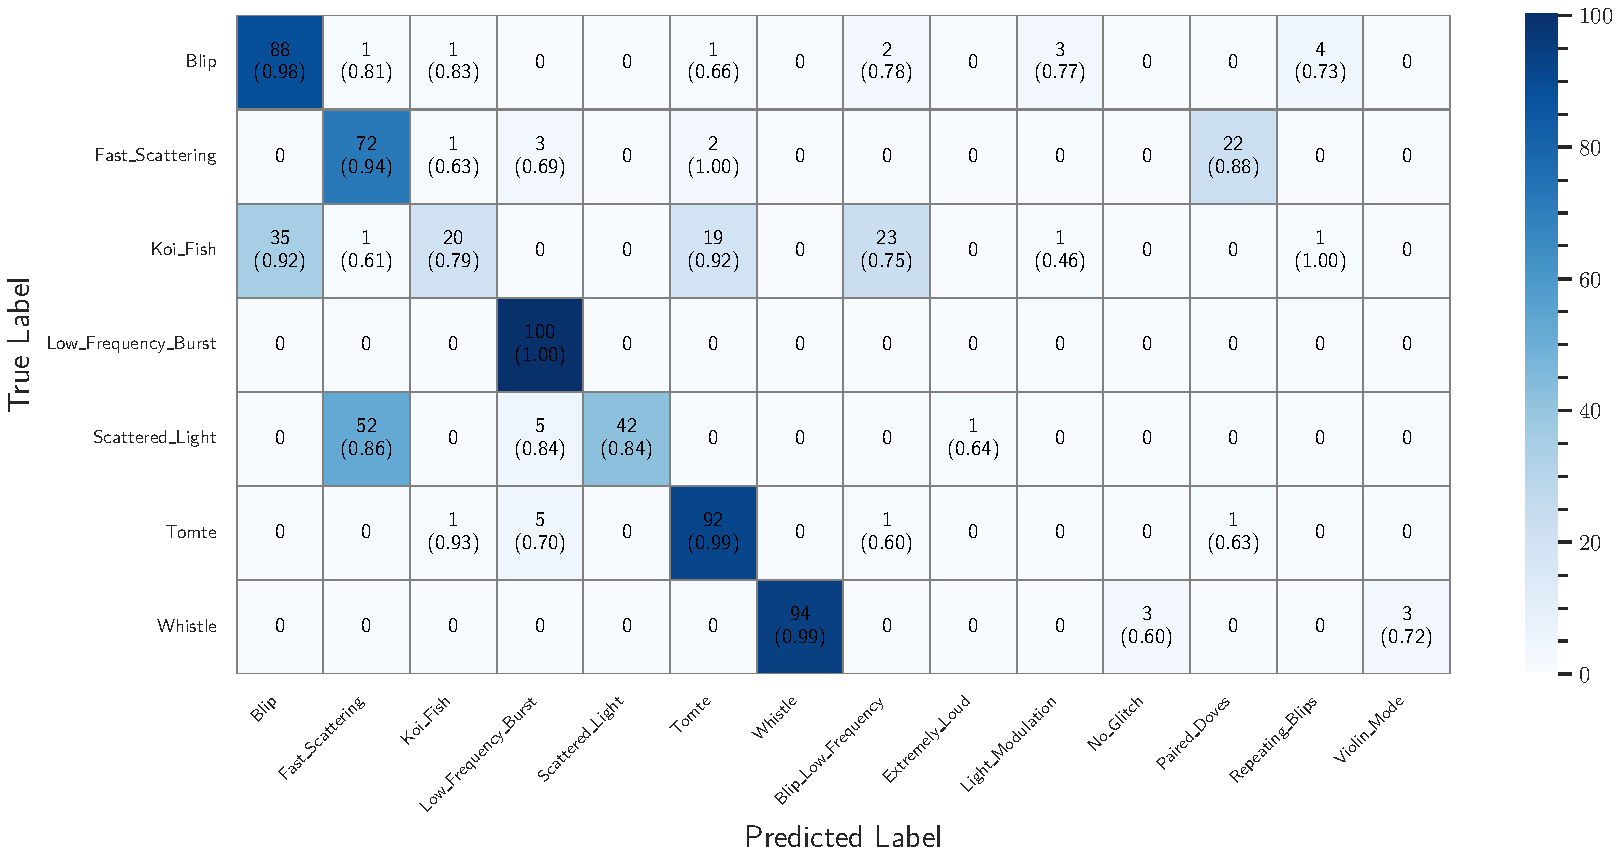
\includegraphics[width=0.8\linewidth]{figures/cDVGAN_CM_confidence.pdf}
\caption[Gravity Spy classification of synthetic GlitchGAN glitches]{
Confusion matrix showing Gravity Spy classifications of glitches generated by GlitchGAN, with 100 samples per class.
Each cell indicates the number of samples predicted for each class, with the average Gravity Spy confidence shown in brackets.s
The strong diagonal structure demonstrates that most synthetic glitches are correctly classified according to their intended class.}
\label{fig:cDVGAN_CM}
\end{figure*}

The resulting confusion matrix (Figure~\ref{fig:cDVGAN_CM}) shows:

\begin{enumerate}
\item
\textbf{Overall accuracy:} $\sim 72\%$ on the full confusion matrix

\item
\textbf{Per-class performance:}
Blip (92\%), Fast Scattering (87\%), Scattered Light (82\%, with misclassifications mostly as Fast Scattering---morphologically reasonable), Tomte (78\%), Whistle (94\%).

\item
\textbf{Problematic classes:} 
Koi Fish shows the lowest per-class accuracy at $\sim 20\%$, but most misclassifications are to morphologically similar classes (Blip, Blip Low Frequency, Tomte), which is consistent with known limitations of Gravity Spy for these morphologically proximate classes.

\end{enumerate}

To understand SNR dependencies, we also tested glitch injection at SNR = 20 and SNR = 150.
At SNR = 150, Koi Fish classification accuracy rises to 79\%, and Whistle accuracy remains at 96\%.
At SNR = 20, Koi Fish shows near-zero accuracy (mostly misclassified as Blip), and Whistle shows frequent misclassification as No Glitch.

This strong SNR dependence suggests that:
(i) Gravity Spy operates primarily on magnitude-level morphological cues (via $Q$-transform magnitude spectrograms)
(ii) Phase information and waveform details matter significantly for morphological characterization
(iii) The synthetic morphologies are realistic within the SNR regimes for which the classifier was trained

\subsection{Global morphological similarity via UMAP}

To assess whether GlitchGAN captures the overall structure of the real glitch distribution, we project both real and synthetic glitch samples into a three-dimensional latent space using UMAP \citep{McInnes_2018}.

\begin{figure*}[t]
\centering
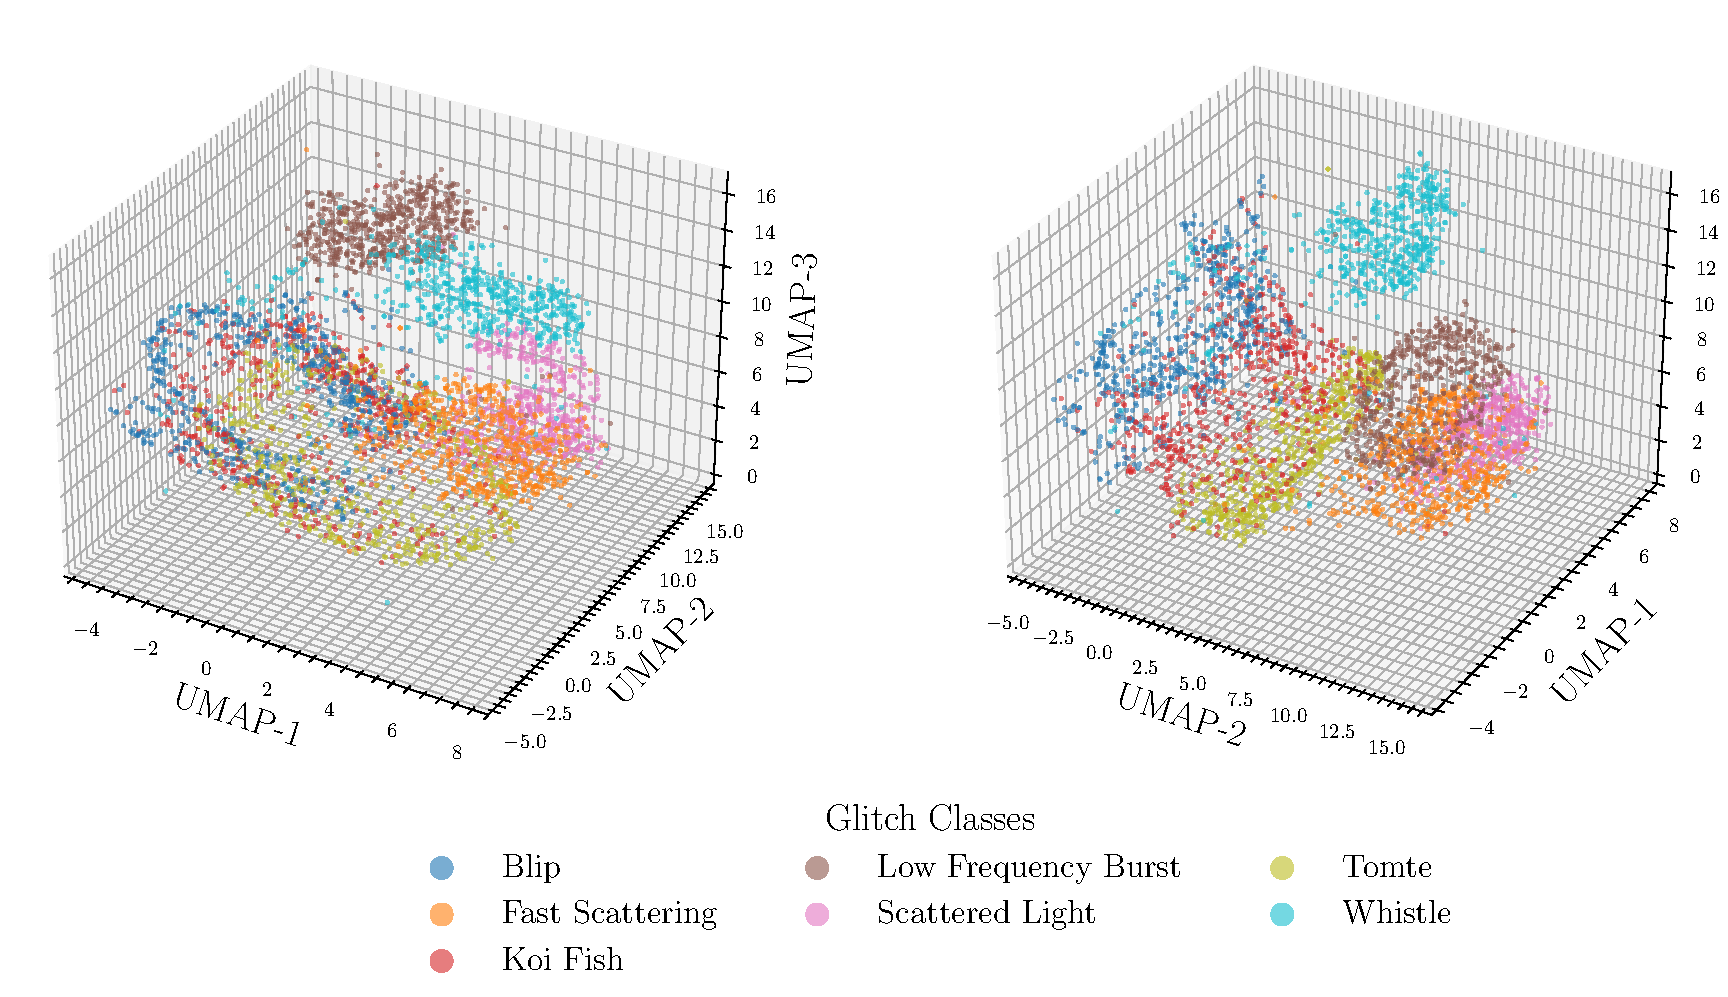
\includegraphics[width=\linewidth]{figures/umap_two_views_axis_swapped_corr.pdf}
\caption[Two perspectives of 3D UMAP embeddings comparing real and generated glitches]{
Two complementary 3D views of the UMAP embeddings showing real and generated glitch samples.
Each color corresponds to one of the seven glitch classes used during training.}
\label{fig:umap_two_views}
\end{figure*}

Figure~\ref{fig:umap_two_views} shows two complementary 3D perspectives of this embedding space, computed from 500 samples per class.
Corresponding individual class-wise UMAP projections (Figure~\ref{fig:umap_per_class_rotated}) provide additional detail.
Strong overlap between real (blue) and synthetic (green) samples indicates that GlitchGAN has learned the general morphological structure of the different glitch types.

For most classes (Blip, Fast Scattering, Scattered Light, Tomte), synthetic and real samples show close clustering with substantial overlap.
The Whistle class exhibits the most noticeable divergence, with synthetic samples forming a partially separate cluster, suggesting that GlitchGAN captures the dominant Whistle morphology but does not fully explore the full morphological diversity within this class.
This is consistent with the relative complexity of the Whistle waveform structure and may reflect limitations of the fixed GAN architecture when applied to this particular class without hyperparameter tuning.

\begin{figure*}[t]
\centering
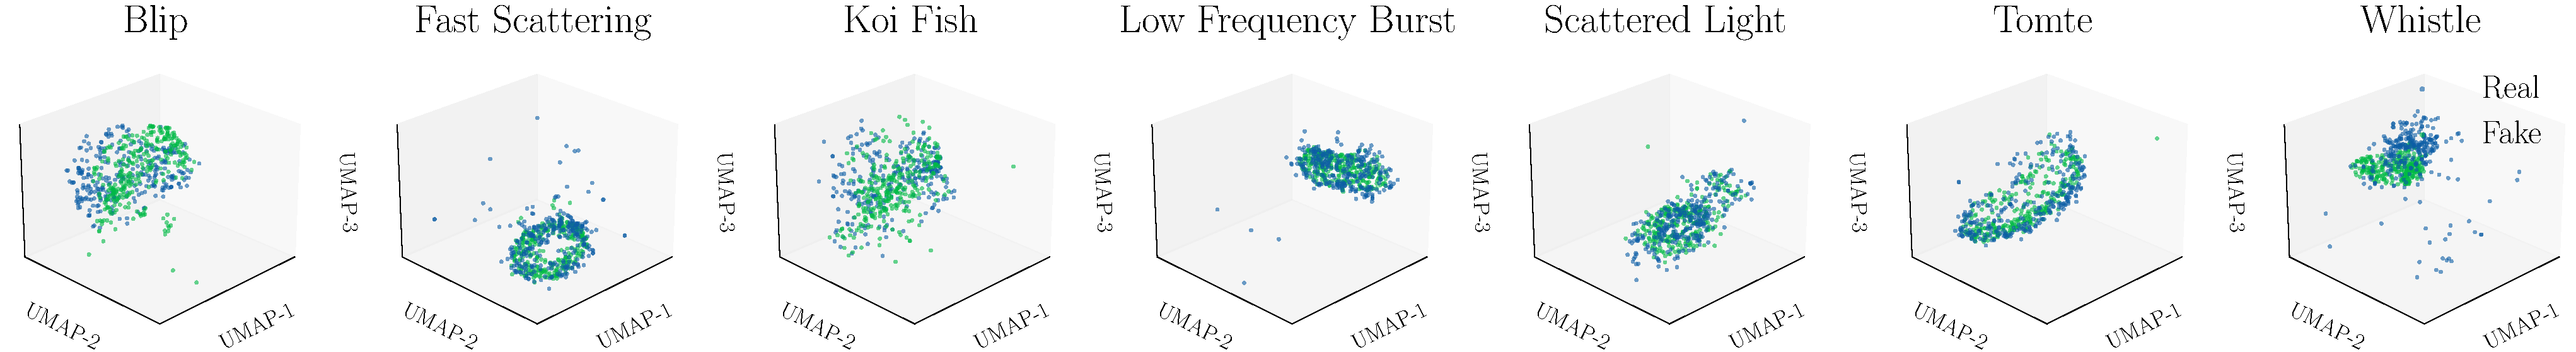
\includegraphics[width=\linewidth]{figures/umap_per_class_rotated_highres_small.pdf}
\caption[Per-class UMAP embeddings of real and synthetic glitches]{
Three-dimensional UMAP embeddings for each glitch class, comparing real (blue) and GlitchGAN-generated (green) samples.
Each panel corresponds to one glitch type and is shown from a rotated viewpoint to highlight intra-class structure.
The close overlap between real and synthetic distributions across most classes demonstrates that GlitchGAN effectively learns class-specific morphological features, though some variation remains for more complex glitch morphologies.}
\label{fig:umap_per_class_rotated}
\end{figure*}

\subsection{Generating hybrid glitches via class interpolation}

A key advantage of class-conditional generative models is the ability to produce ``hybrid'' or transitional morphologies by sampling mixed class vectors.

We explore two sampling strategies:

\begin{enumerate}
\item
\textbf{Simplex mixing:} The class vector is normalized such that all coefficients sum to 1, i.e., sampled from a $k=7$ simplex. This constrains mixing proportions to sum to 100\%.

\item
\textbf{Uniform mixing:} Each class coefficient is independently sampled from $[0, 1]$ without normalization constraint, allowing more extreme interpolations.
\end{enumerate}

\begin{figure*}[t]
\centering
% ---------- (a) Simplex Mixing ----------
\begin{subfigure}[t]{0.48\linewidth}
    \centering
    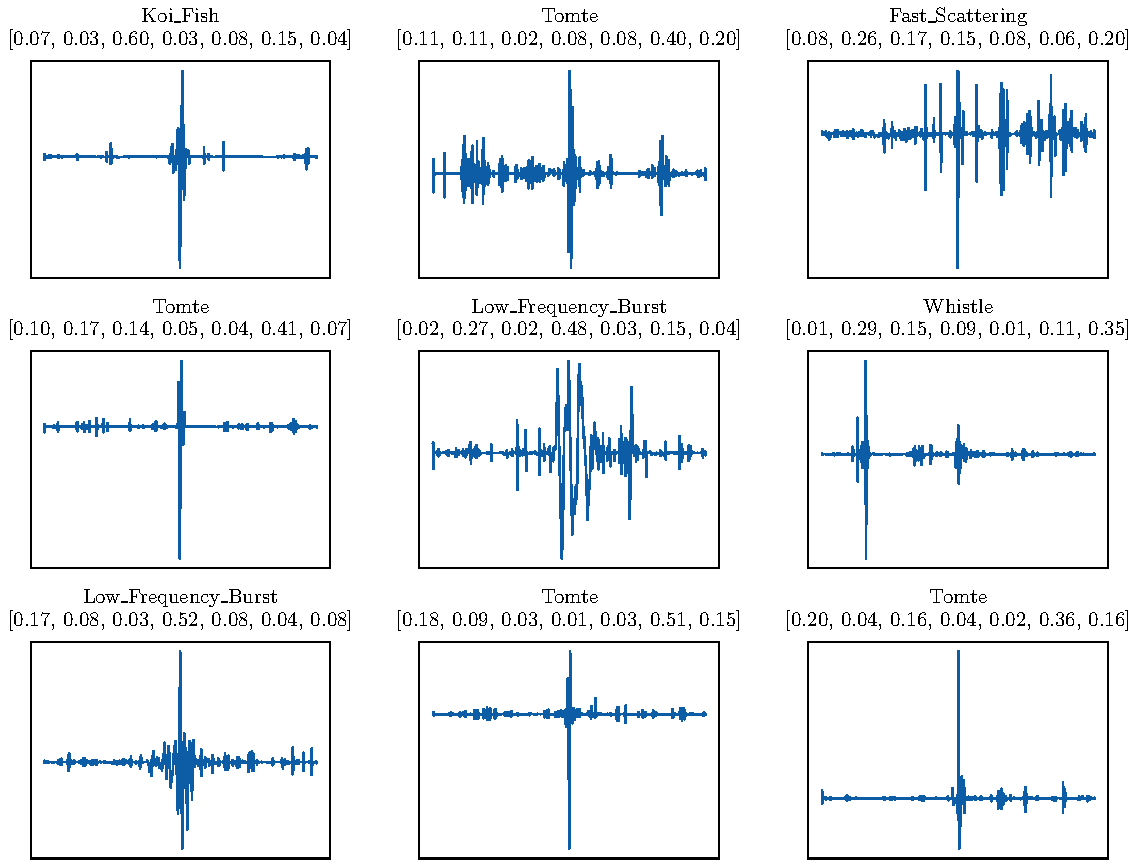
\includegraphics[width=\linewidth]{figures/generated_glitches_simplex_mixing.pdf}
    \caption{Simplex mixing ($\sum c_i = 1$).}
    \label{fig:mixing_simplex}
\end{subfigure}
\hfill
% ---------- (b) Uniform Mixing ----------
\begin{subfigure}[t]{0.48\linewidth}
    \centering
    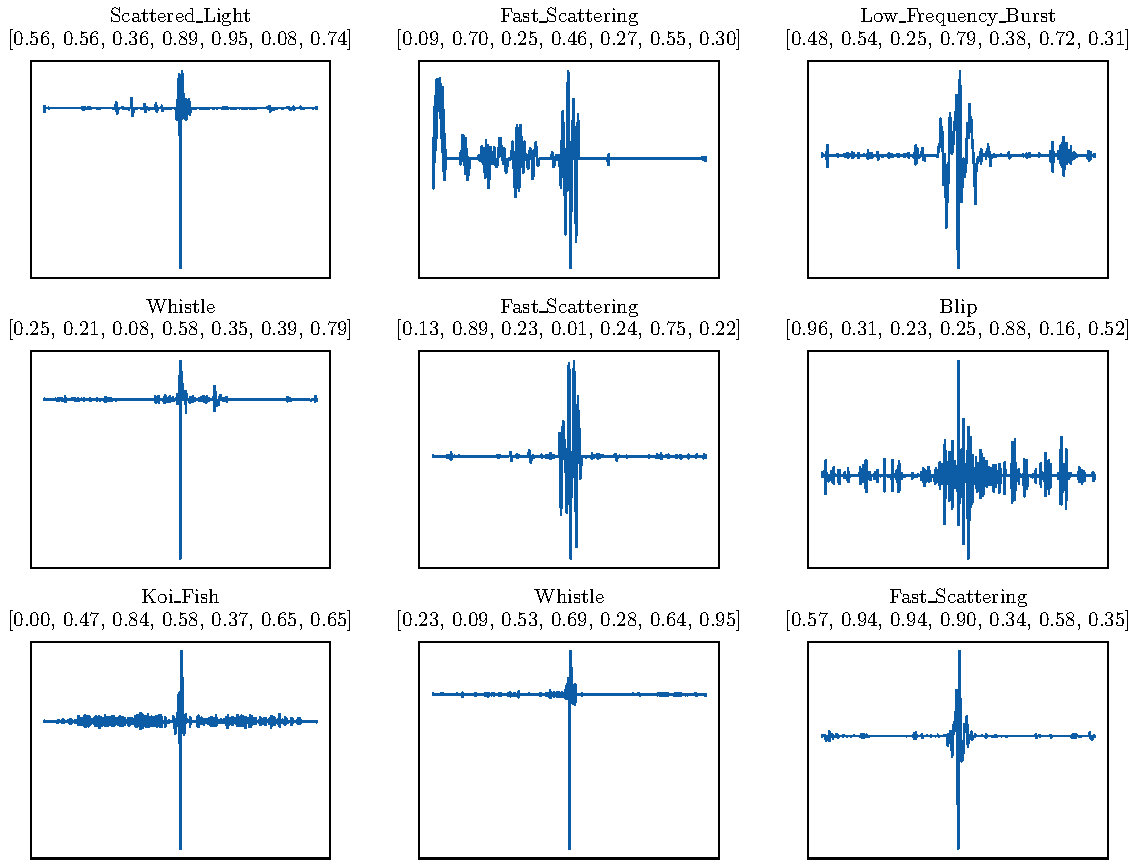
\includegraphics[width=\linewidth]{figures/generated_glitches_uniform_mixing.pdf}
    \caption{Uniform mixing ($c_i \in [0,1]$).}
    \label{fig:mixing_uniform}
\end{subfigure}

\caption[Hybrid glitch generation via class-conditioned mixing]{
Examples of hybrid glitch waveforms generated by GlitchGAN using two class-conditioning strategies.
\textbf{(a)} Simplex mixing samples each class vector from $k=7$ simplex, ensuring coefficients sum to one.
\textbf{(b)} Uniform mixing samples each coefficient independently from a uniform distribution in U$[0, 1]$.
The corresponding sampled class vectors are shown above each plot, with the dominant glitch label also shown. Both methods produce hybrid morphologies interpolating between glitch classes, demonstrating GlitchGAN's ability to explore smooth transitions across the learned latent class space.}
\label{fig:hybrid_glitch_mixing}
\end{figure*}

Figure~\ref{fig:hybrid_glitch_mixing} shows waveform examples from both mixing strategies, demonstrating realistic intermediate morphologies.
The UMAP projection of mixed samples (Figure~\ref{fig:simplex_uniform_umap}) confirms that these hybrid samples smoothly interpolate between pure-class point clouds, with uniform mixing exploring the broadest region of morphospace.

\begin{figure}[ht]
\centering
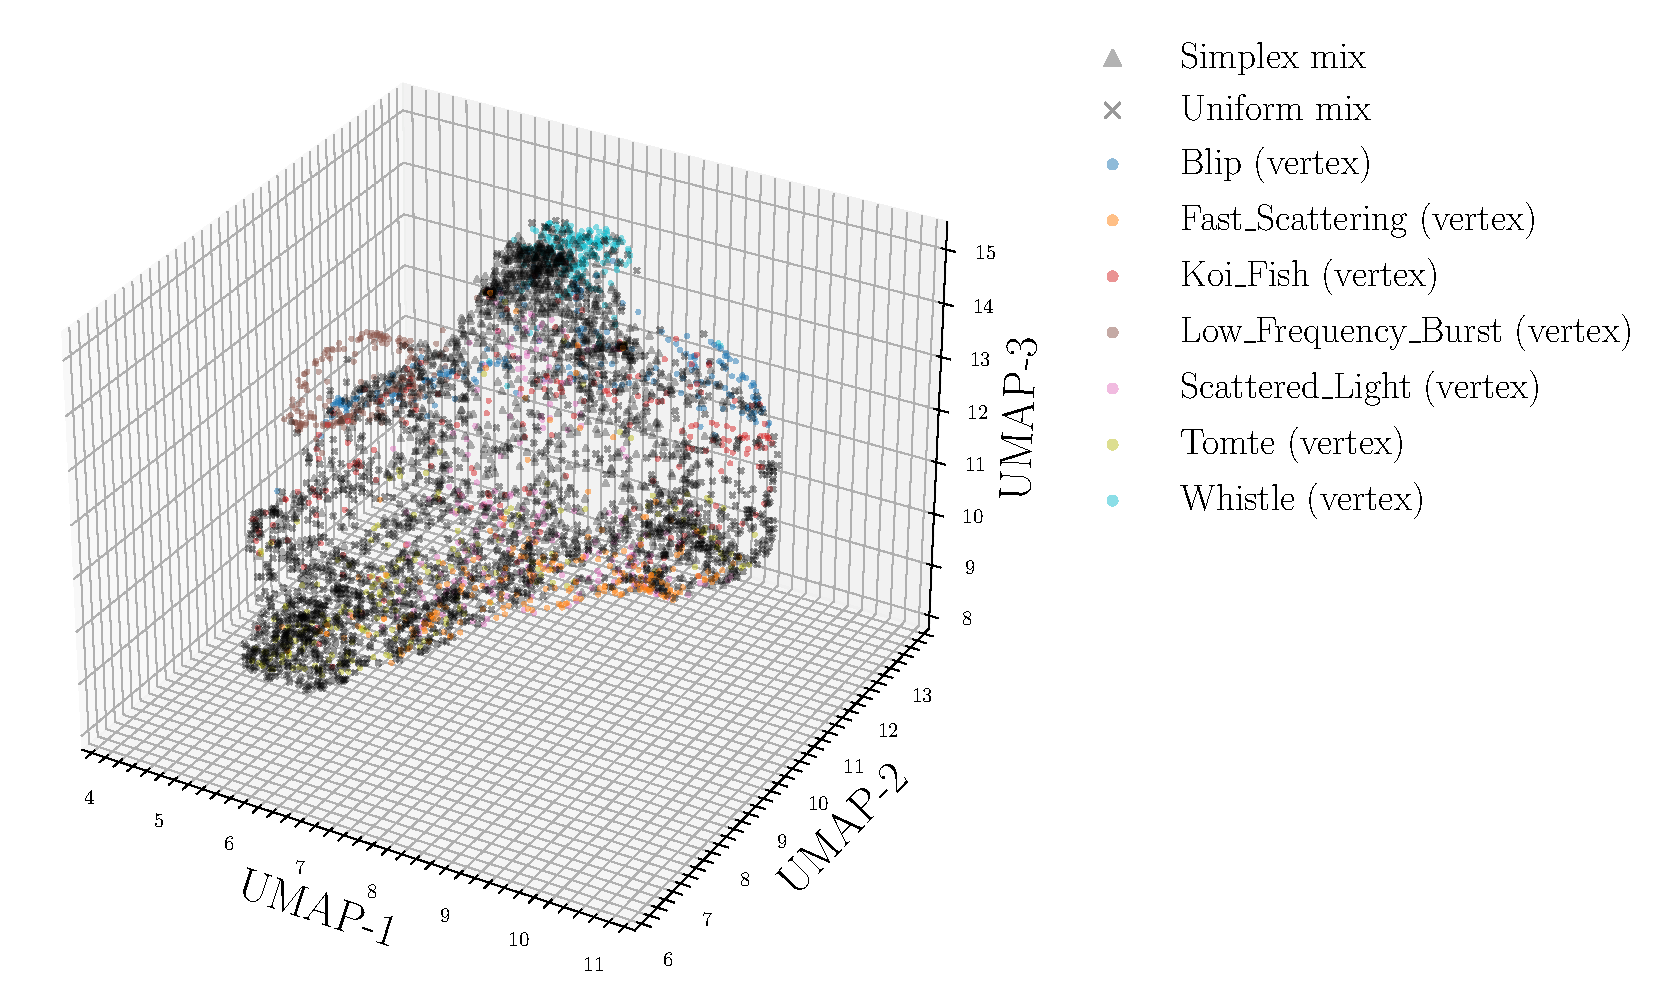
\includegraphics[width=\linewidth]{figures/simplex_uniform_vertex_subsampled_umap_small.pdf}
\caption[UMAP embedding of class-mixed and vertex glitch samples]{
Three-dimensional UMAP embedding showing the distribution of class-mixed glitch samples relative to the vertex (pure-class) glitches.
Vertex samples are colored by their respective glitch class, while class-mixed samples generated using simplex and uniform class-conditioning vectors are shown in black.
The smooth interpolation of mixed samples between class clusters illustrates how GlitchGAN captures continuous transitions across glitch morphologies in the latent class space, spanning the diversity of glitch types represented in the training set.}
\label{fig:simplex_uniform_umap}
\end{figure}

While hybrid samples are not further analyzed in this study, they have potential applications for pipeline robustness testing and data augmentation for classification systems.


\subsubsection{Limitations of magnitude-only representations}

We further evaluated the DiT model (Figures~\ref{fig:dit_umap} and~\ref{fig:dit_confusion}).
DiT-generated samples overlap with real glitches primarily for low-frequency classes (e.g., Fast Scattering, Scattered Light), but show reduced diversity and separable clusters for most other classes where GlitchGAN was more successful.
Remarkably, when these DiT-generated glitches were classified by Gravity Spy at SNR = 50, the classifier confidently assigned them to the correct classes with high confidence scores, despite UMAP clearly showing them to be morphologically distinct from real glitches.

\begin{figure}[ht]
\centering
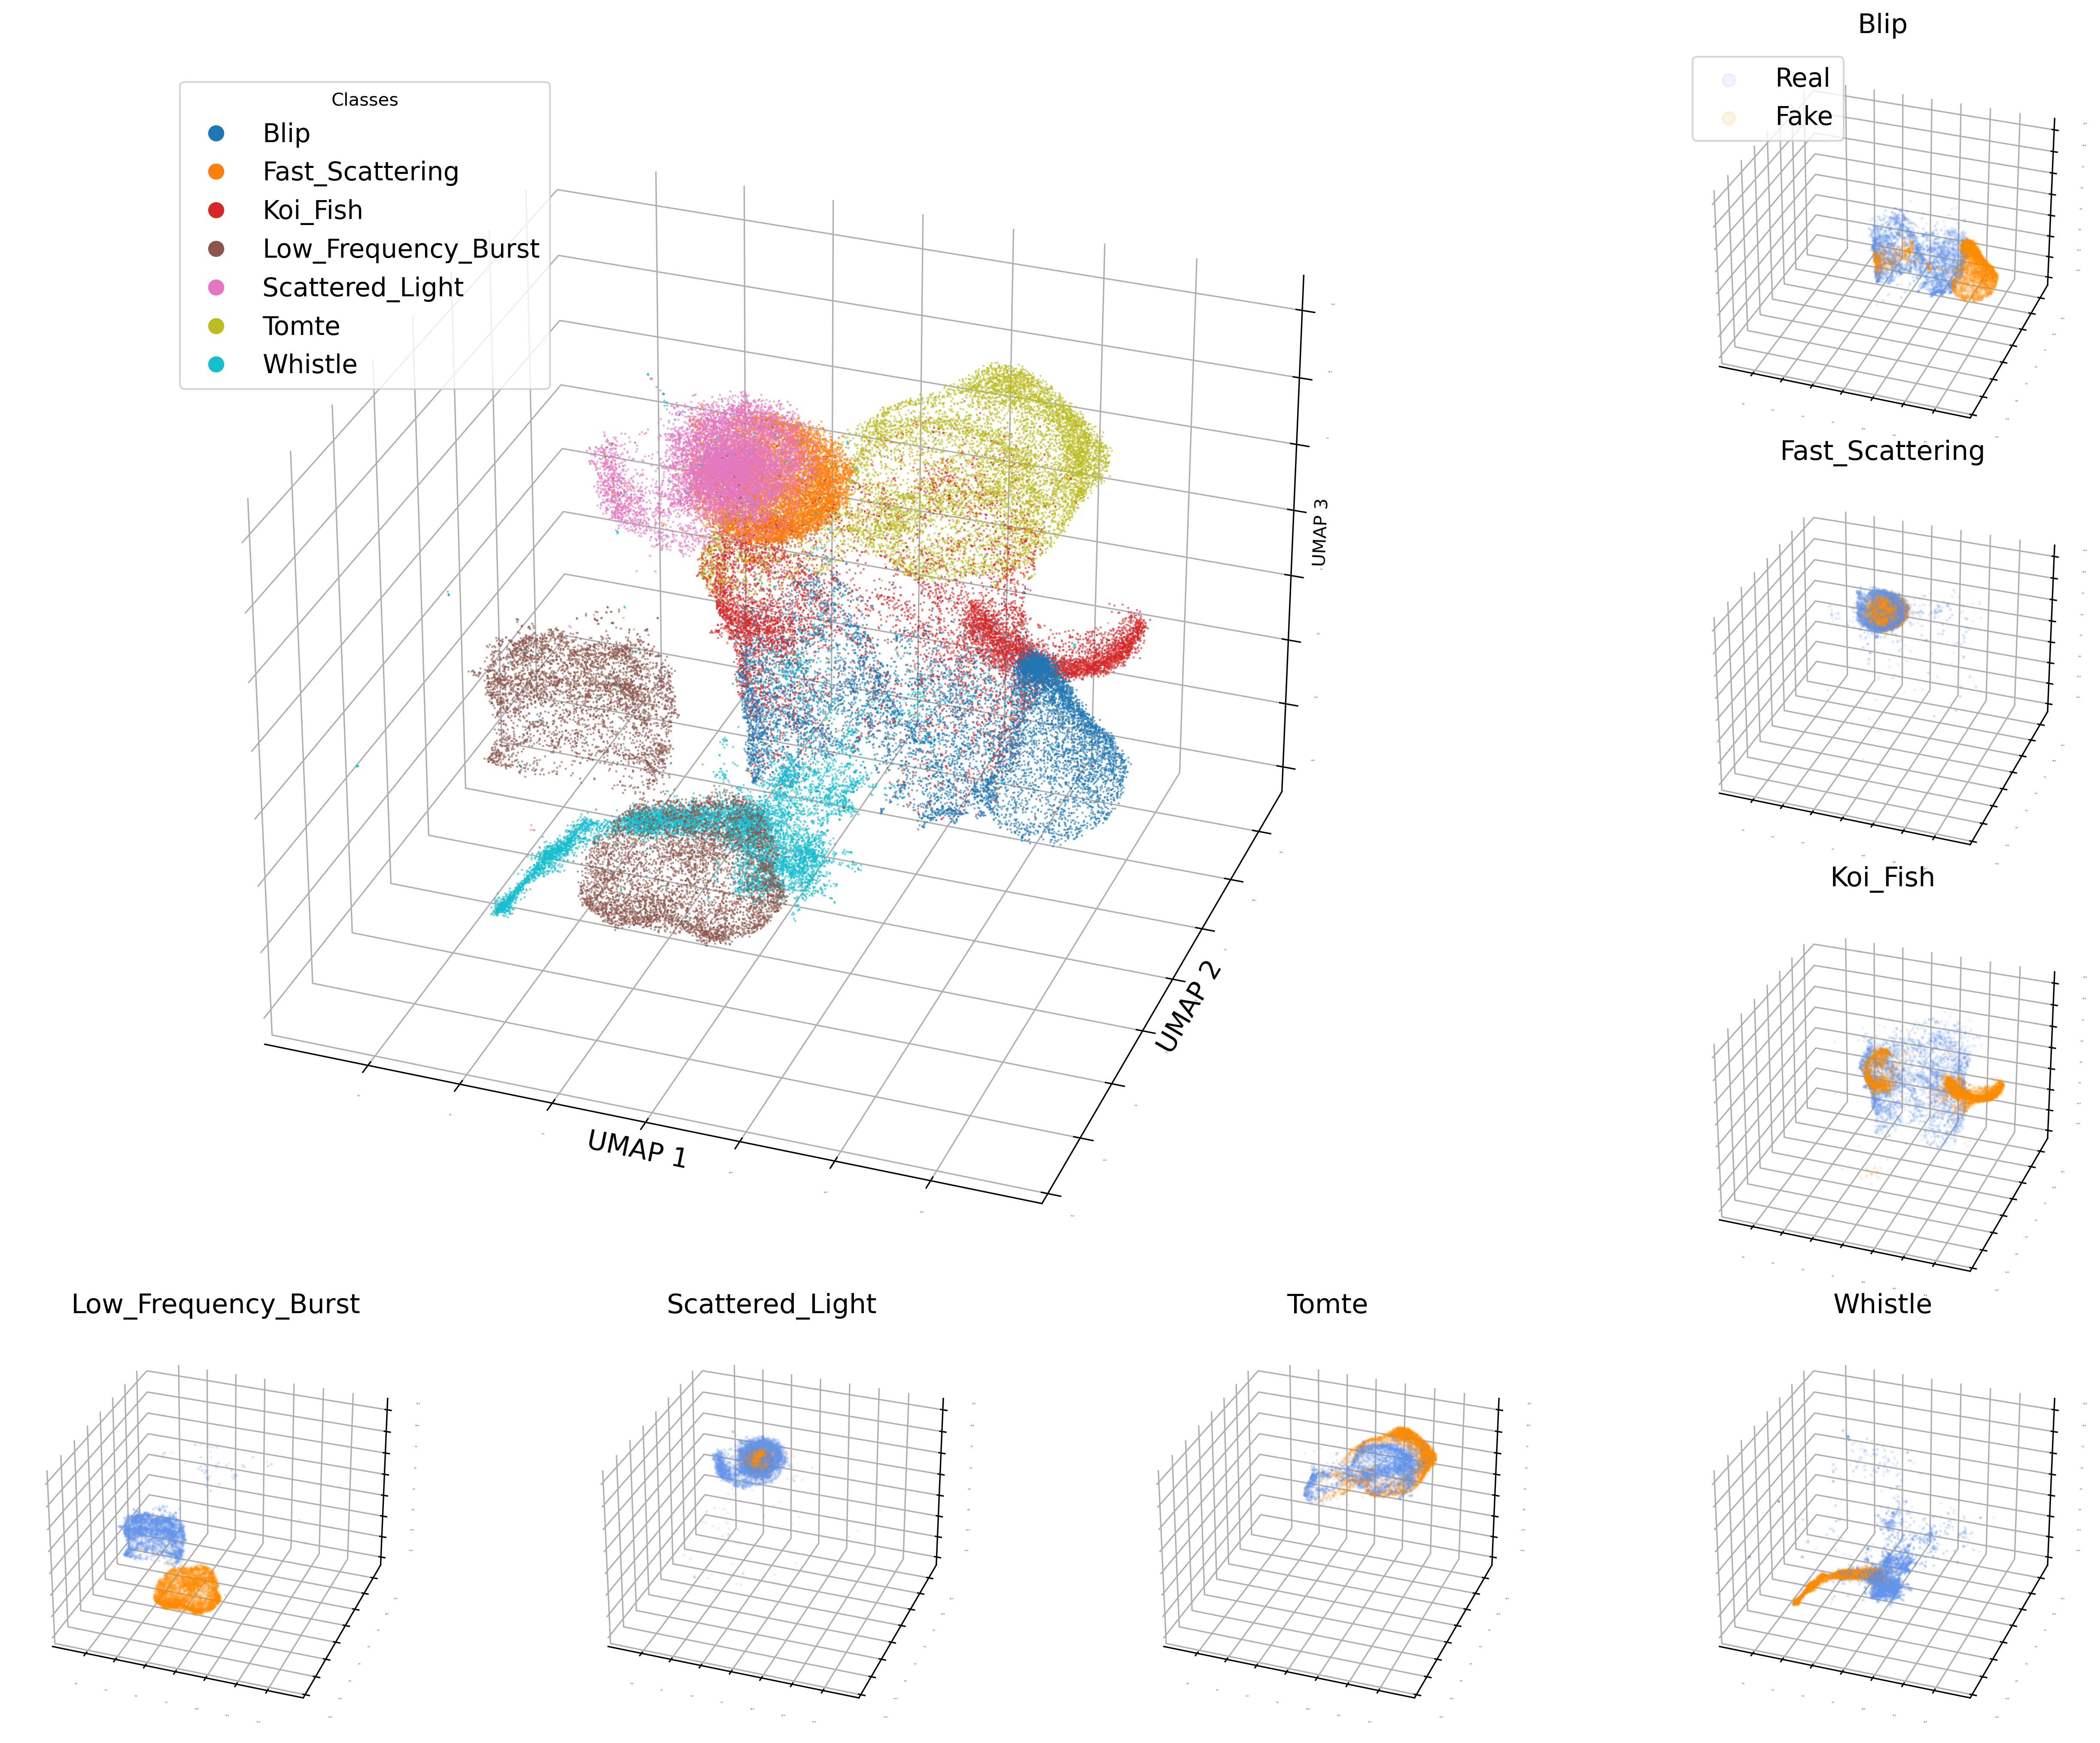
\includegraphics[width=\linewidth]{figures/dit_umap_comparison.png}
\caption{Three-dimensional UMAP projection of real (orange) and DiT-generated (blue) glitches across all seven classes. The large panel shows the overall structure, while smaller panels display each class individually. Overlapping clusters indicate morphological similarity between real and synthetic samples; separable clusters for most classes indicate that DiT does not reproduce the full morphological structure of real glitches, in contrast to GlitchGAN (Figure~\ref{fig:umap_two_views}).}
\label{fig:dit_umap}
\end{figure}

\begin{figure}[ht]
\centering
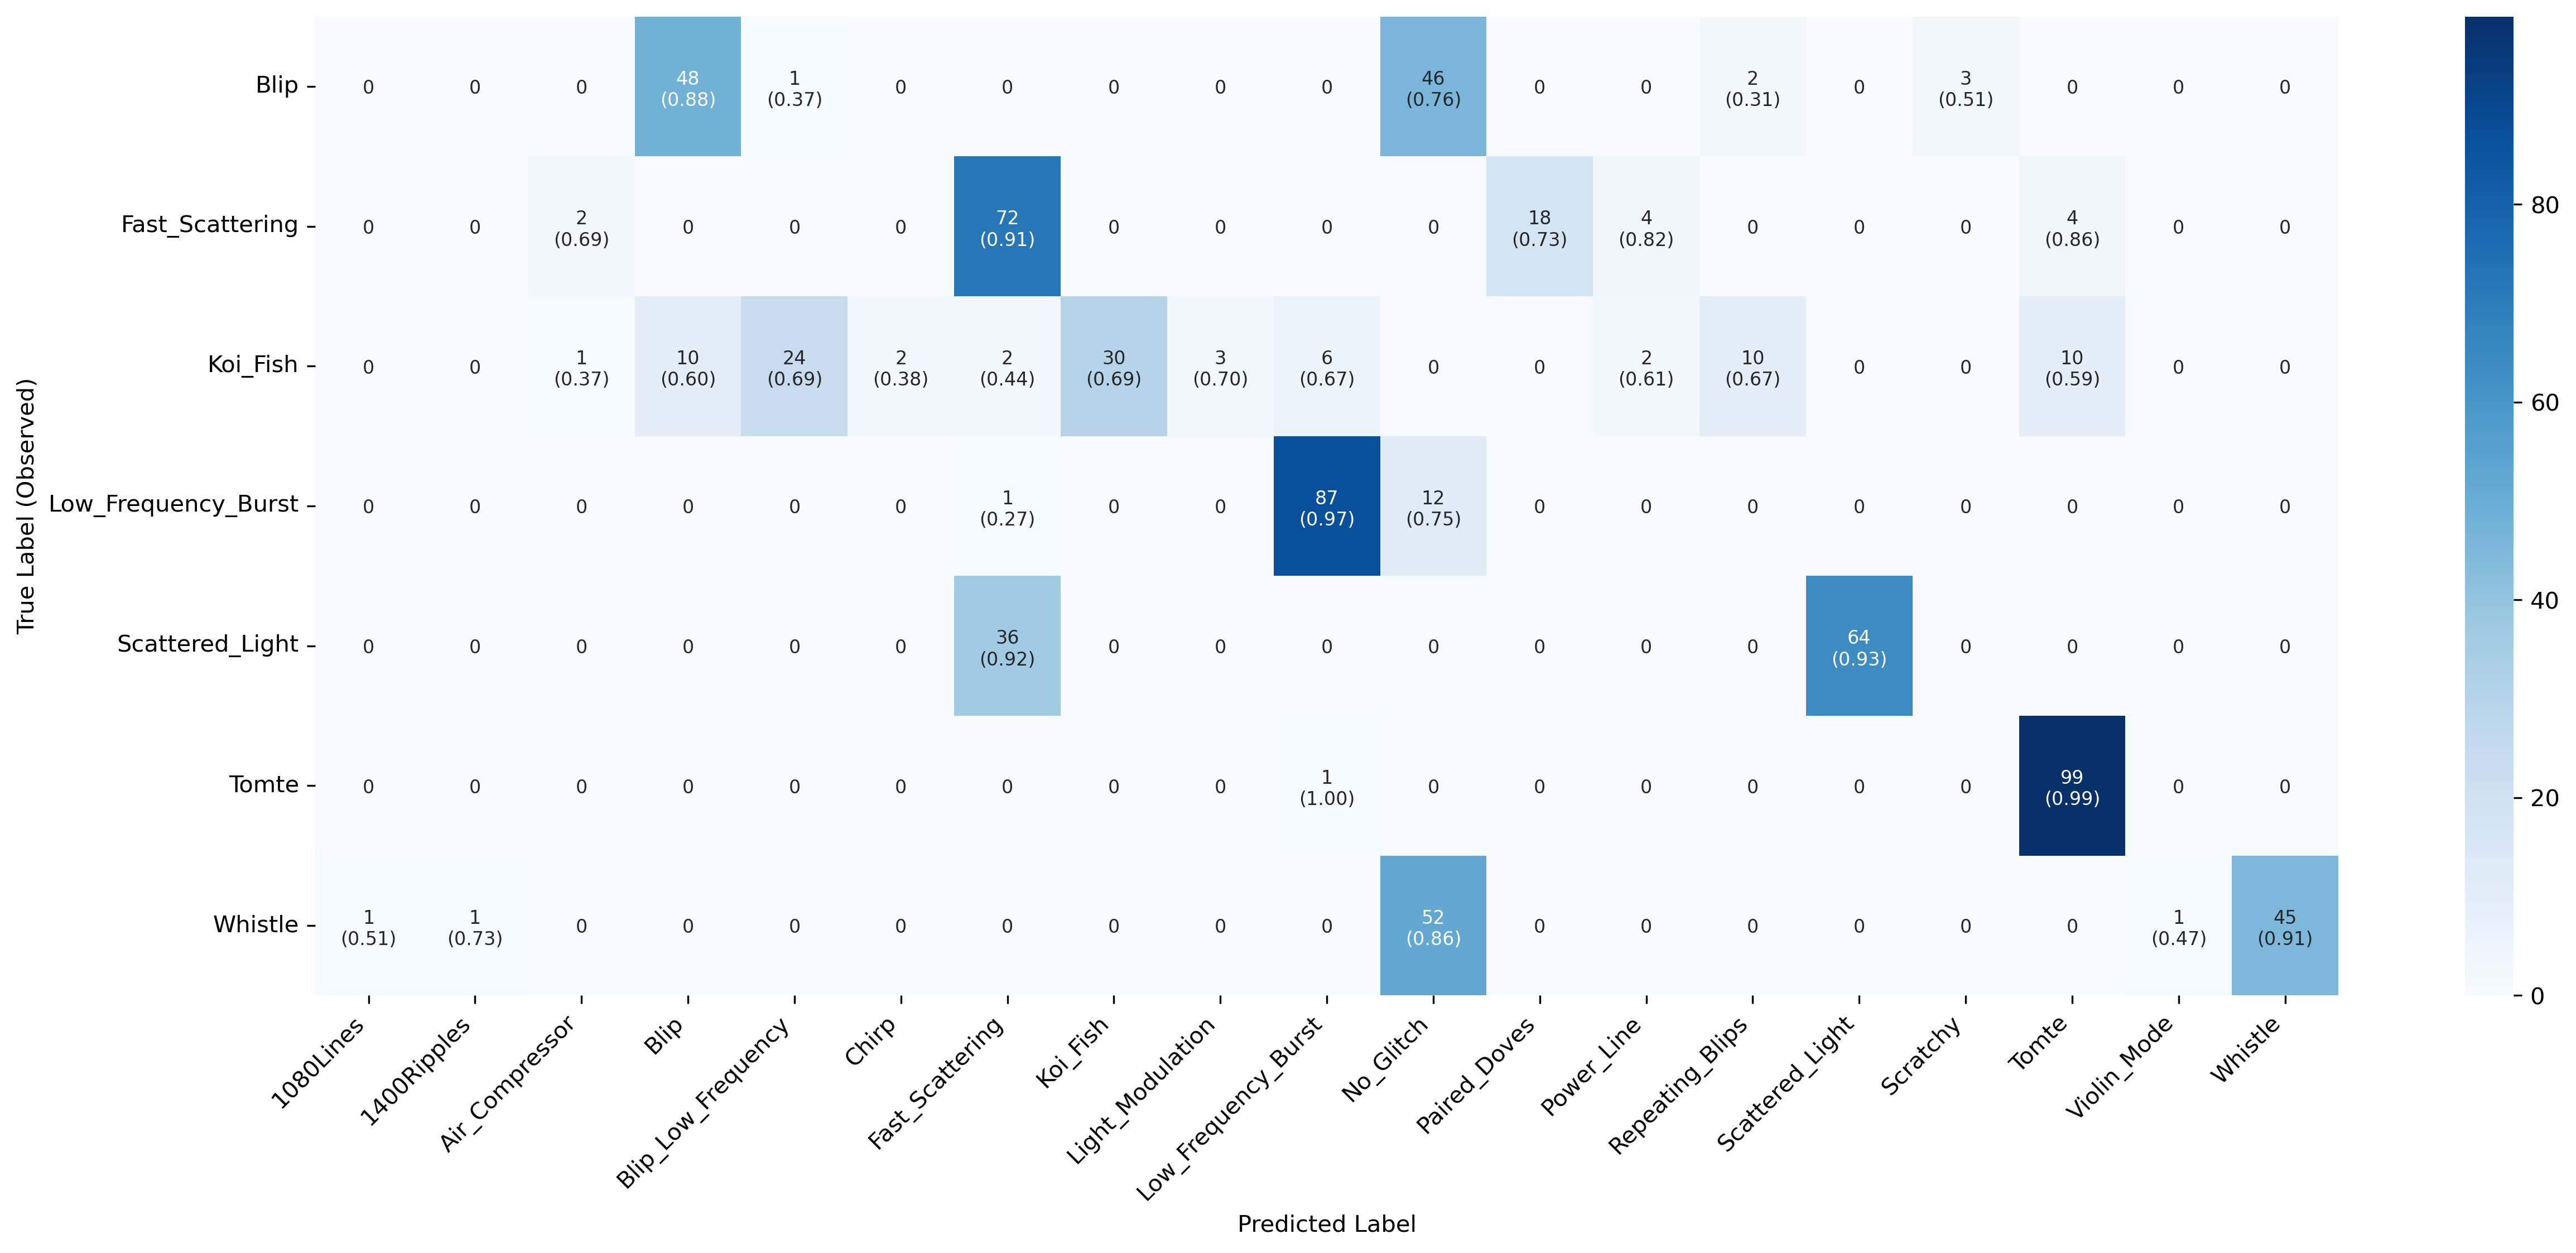
\includegraphics[width=\linewidth]{figures/dit_confusion_matrix.png}
\caption{Gravity Spy confusion matrix for samples generated by the DiT model (100 per class). Each cell shows the number of predictions and mean classifier confidence in brackets. Despite the poor UMAP overlap, Gravity Spy achieves high confidence classification for most classes, illustrating the limitation of magnitude-only validation.}
\label{fig:dit_confusion}
\end{figure}

A notable example is the Low Frequency Burst class: UMAP reveals two clearly distinct clusters (real vs.\ synthetic), yet Gravity Spy classifies 87\% of DiT-generated samples correctly with 97\% mean confidence.
Figure~\ref{fig:dit_lfb} illustrates why: while the time-domain waveforms of real and DiT-generated Low Frequency Bursts are clearly distinct, their magnitude $Q$-scan representations appear similar, explaining the classifier's high confidence despite the physically unrealistic time-domain morphology.

\begin{figure}[ht]
\centering
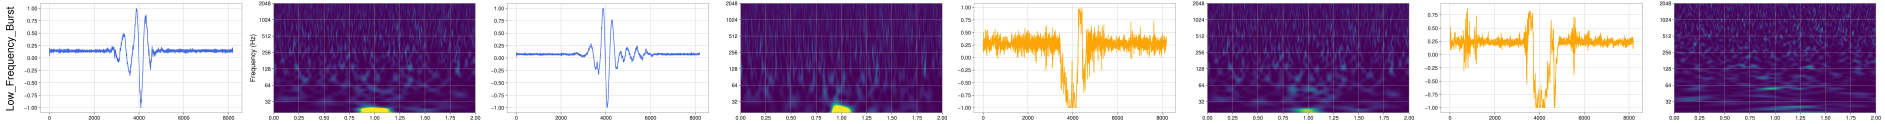
\includegraphics[width=\linewidth]{figures/dit_low_freq_burst_comparison.png}
\caption{Two examples each of real (left) and DiT-generated (right) Low Frequency Burst glitches, showing both the time-domain waveform and the magnitude $Q$-scan representation. The time-domain waveforms are clearly distinct, yet the $Q$-scans appear similar---explaining why Gravity Spy classifies the DiT samples correctly with high confidence despite their physical unrealism.}
\label{fig:dit_lfb}
\end{figure}

This discrepancy arises because the $Q$-transform used by Gravity Spy operates on magnitude-only spectrograms, discarding all phase information.
A less robust generative model may produce synthetic glitches with realistic magnitude-level morphology (e.g., correct duration, central frequency, and bandwitdh) while having fundamentally incorrect phase relationships.

This finding underscores a critical limitation: \textbf{classifiers operating on magnitude-only representations cannot reliably assess glitch realism}.
Complementary validation methods preserving phase information (such as UMAP on time-domain waveforms) are essential for ensuring synthetic glitches are suitable for detector simulations.

Overall, while the DiT model demonstrates that latent diffusion is a viable approach to conditional time-domain glitch generation, its ability to reproduce full morphological diversity---especially for mid- and high-frequency content---is limited relative to GlitchGAN when evaluated out of the box.

\section{Discussion}
\label{sec:discussion}

\subsection{Performance assessment and limitations}

GlitchGAN successfully demonstrates time-domain synthesis of multiple realistic glitch classes.
Substantial UMAP overlap between real and synthetic samples, combined with per-class Gravity Spy accuracies exceeding 90\% (for well-characterized classes), indicates genuine morphological fidelity.

Limitations include:
\begin{enumerate}
\item
Partial failure on the Whistle class, possibly due to insufficient regularization or architectural constraints on receptive field size

\item
SNR-dependent performance of Gravity Spy, requiring careful attention to injection conditions when using these samples in simulations

\item
Normalization to a single effective SNR scale, requiring post-generation rescaling for applications

\item
No hyperparameter optimization for this specific dataset---the model is evaluated ``out-of-the-box'', representing a conservative assessment of GlitchGAN's potential
\end{enumerate}

\subsection{Physics and generative modeling implications}

The diversity of glitch morphologies reflects distinct physical mechanisms~\cite{LIGO_second_third_detchar, Virgo_detchar_O3}.
That a single model can capture this diversity suggests these mechanisms produce outputs that, while distinct, share sufficient structural regularity to be learned by a single generator.
Conversely, the partial failure on Whistle suggests that this class may involve either (i) qualitatively distinct physics, (ii) greater morphological heterogeneity within the class, or (iii) features that are difficult to represent given our network architecture.

Future work incorporating attention mechanisms, dilated convolutions for multi-scale feature extraction, or architecture search could improve performance.

\subsection{Practical applications}

The synthetic glitch population produced by GlitchGAN is immediately useful for:

\begin{enumerate}
\item
\textbf{Mock data challenges (MDCs):} Enriching realistic detector simulations with synthetic instrumental noise, enabling robustness testing of analysis pipelines

\item
\textbf{Detector characterization:} Validating glitch detection, mitigation, and subtraction algorithms

\item
\textbf{Training data augmentation:} Supplementing limited real glitch samples for machine learning algorithms, especially for rare glitch classes

\item
\textbf{Pipeline robustness testing:} Assessing detector sensitivity and false-alarm rates in the presence of instrumental noise morphologies
\end{enumerate}

\subsection{Recommendations for future work}

\begin{enumerate}
\item
Hyperparameter optimization and architectural refinements specifically targeting the Whistle and Koi Fish classes

\item
Incorporation of additional glitch classes (e.g., Blip Low Frequency, Extremely Loud) to cover fuller ranges of detector noise

\item
Development of more sophisticated validation metrics that explicitly evaluate phase consistency, not just magnitude-level morphology

\item
Conditional generation strategies allowing control over glitch duration, SNR, and frequency content independently from class morphology

\item
Extension to multi-detector synthesis, capturing correlations between LIGO Hanford and Livingston glitch populations

\item
Integration with mock data challenge pipelines for rapid deployment in detector simulations
\end{enumerate}

\section{Conclusions}

We have demonstrated that class-conditional deep generative models can effectively synthesize realistic gravitational-wave detector glitches directly in the time domain.
By leveraging high-fidelity DeepExtractor reconstructions and training a single unified model based on the cDVGAN architecture across seven glitch classes, we achieve synthetic samples with strong morphological agreement with real data.

Our multi-faceted validation approach---combining unsupervised latent-space analysis and supervised classification---reveals the method's capabilities while highlighting a critical methodological insight: magnitude-only representations (such as $Q$-scans) are insufficient for assessing synthetic glitch realism.
Phase information is essential, and complementary validation approaches are necessary.

The resulting synthetic glitch population offers practical utility for mock data challenges, detector characterization studies, and validation of detection pipelines.
As gravitational-wave detector networks mature and sensitivity improves, the ability to generate realistic instrumental noise backgrounds will become increasingly valuable for characterization and analysis algorithm development.

\section*{Acknowledgements}

% We acknowledge the Gravity Spy citizen science project for providing the foundational glitch classifications used to curate our training data.
% We thank the LIGO Scientific Collaboration for access to detector data through the Gravitational Wave Open Science Center (GWOSC).
% DeepExtractor development was supported by [FUNDING\_ACKNOWLEDGEMENT].

This research has made use of data or software obtained from the Gravitational Wave Open Science Center (gwosc.org), a service of the LIGO Scientific Collaboration, the Virgo Collaboration, and KAGRA. This material is based upon work supported by NSF's LIGO Laboratory which is a major facility fully funded by the National Science Foundation, as well as the Science and Technology Facilities Council (STFC) of the United Kingdom, the Max-Planck-Society (MPS), and the State of Niedersachsen/Germany for support of the construction of Advanced LIGO and construction and operation of the GEO600 detector. Additional support for Advanced LIGO was provided by the Australian Research Council. Virgo is funded, through the European Gravitational Observatory (EGO), by the French Centre National de Recherche Scientifique (CNRS), the Italian Istituto Nazionale di Fisica Nucleare (INFN) and the Dutch Nikhef, with contributions by institutions from Belgium, Germany, Greece, Hungary, Ireland, Japan, Monaco, Poland, Portugal, Spain. KAGRA is supported by Ministry of Education, Culture, Sports, Science and Technology (MEXT), Japan Society for the Promotion of Science (JSPS) in Japan; National Research Foundation (NRF) and Ministry of Science and ICT (MSIT) in Korea; Academia Sinica (AS) and National Science and Technology Council (NSTC) in Taiwan.
The authors are grateful for computational resources provided by the LIGO Laboratory and supported by the National Science Foundation Grants No. PHY-0757058 and No. PHY-0823459.
% Finally, we thank the anonymous referees for their useful suggestions in improving the manuscript.

% \section*{Data Availability}

% The synthetic glitch samples generated in this work are available upon request.
% Code for the cDVGAN model and training pipeline is available at [REPOSITORY\_URL].

\bibliography{references}

\end{document}
